% ============================================================================
%  MARS: Memory for Autonomous Real-time Systems
%  A GPU-Resident Retrieval Substrate with Native Temporal Decay
%  and Importance Scoring
%
%  arXiv submission draft — cs.DC with cs.IR cross-listing
%  Antonello Fratepietro, 2026
% ============================================================================
%
%  Build: tectonic --reruns 3 main.tex
%     or: pdflatex main && bibtex main && pdflatex main && pdflatex main
%
%  All experimental results measured on NVIDIA A100 SXM4 80GB and/or
%  RTX 5060 Ti. Same-hardware FAISS/CAGRA comparison on A100 SXM4.
% ============================================================================

\documentclass[11pt]{article}

\usepackage[margin=1in]{geometry}
\usepackage[utf8]{inputenc}
\usepackage[T1]{fontenc}
\usepackage{times}
\usepackage{graphicx}
\usepackage{amsmath}
\usepackage{amssymb}
\usepackage{booktabs}
\usepackage{multirow}
\usepackage{array}
\usepackage{xcolor}
\usepackage{hyperref}
\usepackage{listings}
\usepackage{microtype}
\usepackage{url}
\usepackage{tcolorbox}
\usepackage{pifont}
\usepackage{algorithm}
\usepackage{algorithmic}
\usepackage{amsthm}
\newtheorem{theorem}{Theorem}
\newtheorem{proposition}[theorem]{Proposition}
\newtheorem{definition}[theorem]{Definition}
\newtheorem{lemma}[theorem]{Lemma}

\hypersetup{
    colorlinks=true,
    linkcolor=blue!60!black,
    citecolor=blue!60!black,
    urlcolor=blue!60!black,
    pdftitle={MARS: A GPU-Resident Memory Substrate for Real-Time Embodied AI},
    pdfauthor={Antonello Fratepietro},
}

% ─── Placeholder macro ────────────────────────────────────────────────
\newcommand{\placeholder}[1]{\textcolor{red}{\textbf{[#1]}}}

% ─── Design target macro ─────────────────────────────────────────────
\newcommand{\target}[1]{\textit{target: #1}}

% ─── Listings setup for CUDA / C++ ──────────────────────────────────
\definecolor{codebg}{rgb}{0.97,0.97,0.97}
\definecolor{codekw}{rgb}{0.1,0.2,0.6}
\definecolor{codestr}{rgb}{0.6,0.15,0.15}
\definecolor{codecom}{rgb}{0.3,0.5,0.3}
\lstset{
    backgroundcolor=\color{codebg},
    basicstyle=\ttfamily\footnotesize,
    keywordstyle=\color{codekw}\bfseries,
    stringstyle=\color{codestr},
    commentstyle=\color{codecom}\itshape,
    breaklines=true,
    frame=single,
    framerule=0pt,
    xleftmargin=1em,
    language=C++,
    morekeywords={__global__,__device__,__host__,__shared__,__restrict__,
                  atomicCAS,atomicAdd,atomicMax,__shfl_down_sync,__expf,
                  blockIdx,blockDim,threadIdx,gridDim,int32_t,int64_t,
                  float,constexpr,nullptr,MemoryGraph,DeviceMemoryGraph,
                  QueryResult,RetrievalConfig,RetrievalStats,FrameTimer},
    showstringspaces=false,
    tabsize=4,
    captionpos=b,
}

% ─── MARS macro ──────────────────────────────────────────────────────
\newcommand{\mars}{\textsc{Mars}}

% ─── Title ────────────────────────────────────────────────────────────
\title{\vspace{-1.5cm}\mars{}: A GPU-Resident Retrieval Substrate\\
with Native Temporal Decay\\
for Real-Time Embodied AI}

\author{Antonello Fratepietro\\
\texttt{https://github.com/antonellof/MARS}}

\date{April 2026}

% ══════════════════════════════════════════════════════════════════════
\begin{document}
\maketitle

% ─── Abstract ─────────────────────────────────────────────────────────
\begin{abstract}
Real-time AI systems --- autonomous vehicles, humanoid robots, AR/VR
headsets --- issue memory retrieval queries at sensor rate (30--1000~Hz)
under tight latency budgets. Existing GPU vector search libraries
(FAISS, cuVS) rank by cosine similarity alone. A post-hoc temporal
filter can restore recency awareness, but requires a two-stage
pipeline. We present \mars{}, a GPU-resident retrieval substrate that
integrates temporal decay directly into the GPU retrieval path,
eliminating this second stage at no accuracy cost.

\mars{} (\textbf{M}emory for \textbf{A}utonomous \textbf{R}eal-time
\textbf{S}ystems) stores text, audio, image, and sensor embeddings in
a shared 768-D space as nodes in a Neural Shortcut Network (NSN) with
cross-modal bridges. Retrieval runs as three GPU stages --- cuBLAS
similarity with temporal decay, CUB top-$K$, warp-cooperative BFS ---
entirely on GPU-resident data with zero per-query allocation.

\medskip\noindent\textbf{Key results} (all measured on A100~SXM4, same
hardware as baselines):
\begin{itemize}
\setlength{\itemsep}{1pt}\setlength{\parskip}{0pt}
\item Wall-clock latency 2.2$\times$ FAISS~Flat at $N{=}1$K, converging
  to parity at $N{=}50$K. The gap is a fixed $\sim$0.15~ms overhead
  from temporal decay and BFS, amortized as corpora grow.
\item Temporal Precision@10 = 0.910 in AV perception, matching
  FAISS~Flat with a post-hoc temporal filter (0.910) at essentially
  identical latency (0.26~ms vs.\ 0.25~ms $p99$), without requiring
  the filter stage.
\item All four demonstrator empirical $p99$ deadlines met: AV 0.87~ms
  (budget 1~ms), robot 0.76~ms (budget 1~ms), AR/VR 1.56~ms (budget
  5~ms), voice 0.88~ms (budget 20~ms).
\item cuBLAS + CUB optimization scales to 13M memories at 29~ms $p99$
  on a single 40~GB A100.
\end{itemize}

\noindent \mars{} fills a gap between fast-but-stateless circular
buffers and capable-but-slow vector databases: a GPU-resident retrieval
substrate with native temporal awareness and cross-modal support
operating at sensor-rate latency budgets.

\textbf{Keywords:} real-time systems, temporal decay, GPU memory,
autonomous driving, multimodal retrieval, CUDA, streaming insertion.
\end{abstract}

% ══════════════════════════════════════════════════════════════════════
\section{Introduction}
\label{sec:intro}

\subsection{The Problem: Real-Time Memory Needs Temporal Awareness}

An autonomous vehicle's perception stack runs at 60~Hz. A child's ball
rolls into the road from behind a parked van. Vision alone sees only
the ball. But 600~ms earlier, the vehicle's microphones captured
children's voices from that same direction --- a memory that, if
retrievable now, raises the prior that a child may follow the ball
into the street. The query isn't ``find the most visually similar
memory''; it's ``find any recent sensor evidence, across any modality,
relevant to what's in front of me.'' A voice sample from last week's
drive through a schoolyard has high audio similarity but is useless.
The useful memory is 600~ms old, from a different modality than the
query, and low in cosine similarity compared to countless
irrelevant-but-similar alternatives in the corpus. No ranking by
similarity alone can surface it.

Existing GPU-accelerated vector search libraries ---
FAISS~\cite{faiss}, cuVS CAGRA~\cite{cuvs}, and similar systems ---
optimize exactly that single objective: find the $K$ vectors with
highest cosine similarity to a query. They treat all indexed vectors
as equally valid regardless of age or modality. For static corpora ---
document retrieval, recommendation, image search --- this is the
correct formulation. For streaming sensor data, it is not.

For streaming sensor data, this produces stale results unless the
application adds a post-hoc temporal filter --- a solution that works
(restoring temporal precision to 0.910 in our AV experiment,
Section~\ref{sec:temporal_relevance}) but introduces a two-stage
pipeline. Similarly, streaming insertion requires periodic index
rebuilds on IVF-class indices, adding latency and a staleness window.
In Section~\ref{sec:temporal} we quantify the cost of this indirection
against \mars{}'s native approach: identical temporal precision at
essentially identical latency (0.26~ms vs.\ 0.25~ms $p99$), without
the filter stage.

\subsection{\mars{}: Native Temporal Decay in the GPU Retrieval Path}

\mars{} (\textbf{M}emory for \textbf{A}utonomous \textbf{R}eal-time
\textbf{S}ystems) integrates temporal decay directly into the GPU
retrieval path. Rather than computing cosine similarity alone and
filtering afterward, \mars{} computes a time-decayed score for every
memory as part of the retrieval pipeline:
\[
s(v, q, t_q) = \langle E(v), q \rangle \cdot
  \exp\!\bigl(-\lambda \cdot (t_q - \tau(v))\bigr)
\]
where $\lambda$ is a workload-tunable decay rate. This changes
the ranking \emph{before} top-$K$ selection, ensuring that temporally
relevant results are surfaced without requiring a second pass or index
rebuild.

\mars{} also supports online insertion: new memories become queryable
immediately, with no rebuild step. Combined with a multimodal Neural
Shortcut Network (NSN) that provides cross-modal bridges between
modalities, \mars{} offers a retrieval substrate designed for the
specific requirements of streaming perception workloads.

\subsection{Contributions}

\begin{enumerate}
\item A \textbf{three-way latency comparison} (Section~\ref{sec:temporal})
  --- FAISS cosine-only, FAISS + post-hoc temporal filter, and \mars{}
  with native decay --- showing that \mars{} matches FAISS+filter at
  identical temporal precision (0.910) and essentially identical latency
  (0.26~ms vs.\ 0.25~ms $p99$), without requiring the filter stage.

\item A \textbf{GPU-resident retrieval pipeline} with native temporal
  decay integrated into the retrieval path
  (Section~\ref{sec:architecture}), matching FAISS~Flat at the target
  corpus sizes while adding temporal awareness and cross-modal
  capability, at a $\leq$2$\times$ latency cost at smaller $N$
  (Section~\ref{sec:comparison}).

\item The \textbf{Multimodal Neural Shortcut Network}
  (Section~\ref{sec:nsn}) with cross-modal bridges providing
  bounded-hop structural reachability across modalities
  (constant-work at tested $N$; see Proposition~\ref{prop:bfs} for
  asymptotic caveats).

\item An \textbf{ablation study} (Section~\ref{sec:ablation}) honestly
  characterizing the contribution of each system component at the
  target corpus sizes.

\item \textbf{Four deadline-aware demonstrators}
  (Section~\ref{sec:demos}) --- AV (60~Hz, 1~ms), robot (1~kHz, 1~ms),
  AR/VR (90~Hz, 5~ms), voice (30~Hz, 20~ms) --- all passing $p99$
  budgets on datacenter and consumer GPUs.

\item An \textbf{episode-scoped retrieval contract}
  (Section~\ref{sec:episode_scoped}) for workloads where the active
  track / session / sub-task id is known at query time. On the
  embodied kids-ball corpus with paired probes it delivers
  \textbf{197~$\mu$s $p99$ at $N{=}1$\,M} (13$\times$ vs.\ the global
  path) with a perfect cross-modal hit rate, while remaining
  composable with the global temporal-decay + BFS path for
  cross-episode queries.
\end{enumerate}

% ══════════════════════════════════════════════════════════════════════
\section{Problem Formulation}
\label{sec:formulation}

This section formalizes the multimodal memory retrieval problem and the
temporal and deadline constraints that distinguish this work from
conventional approximate nearest-neighbor search.

\begin{definition}[Multimodal Memory Corpus]
\label{def:corpus}
A multimodal memory corpus is a tuple
$\mathcal{C} = (V, E, \phi, \mu, \tau)$ where:
\begin{itemize}
\item $V = \{v_1, \ldots, v_N\}$ is a set of $N$ memory nodes;
\item $E: V \rightarrow \mathbb{R}^D$ maps each node to an
  L2-normalized embedding, $\|E(v)\|_2 = 1$;
\item $\mu: V \rightarrow \{0, 1, \ldots, M-1\}$ assigns each node a
  modality tag (text${=}0$, audio${=}1$, image${=}2$);
\item $\tau: V \rightarrow \mathbb{R}_{\geq 0}$ assigns each node a
  timestamp;
\item $\phi$ is the NSN graph topology over $V$.
\end{itemize}
\end{definition}

\begin{definition}[Temporally-Decayed Multimodal Retrieval]
\label{def:retrieval}
Given a query embedding $q \in \mathbb{R}^D$ with $\|q\|_2 = 1$, query
timestamp $t_q$, decay rate $\lambda$, and result size $K$, the
retrieval problem is to find:
\[
\mathrm{top}\text{-}K_{v \in V} \; s(v, q, t_q)
\]
where the time-decayed similarity score is:
\[
s(v, q, t_q) = \langle E(v), q \rangle \cdot
  \exp\!\bigl(-\lambda \cdot (t_q - \tau(v))\bigr).
\]
\end{definition}

\begin{definition}[Temporal Relevance]
\label{def:temporal_relevance}
For a retrieval result set $R = \{v_1, \ldots, v_K\}$ over a corpus
with object identities, \emph{Temporal Precision@K} is the fraction of
results whose object identity matches a ground-truth active object
\emph{and} whose timestamp falls within the current tracking window
$[t_q - w, t_q]$:
\[
\mathrm{TP@}K = \frac{|\{v \in R : \mathrm{active}(v) \wedge
  \tau(v) \geq t_q - w\}|}{K}.
\]
\end{definition}

\begin{definition}[Streaming Freshness]
\label{def:freshness}
A retrieval system has \emph{streaming freshness} if a memory inserted
at time $t_i$ is queryable at time $t_i + \epsilon$ for arbitrarily
small $\epsilon > 0$, without requiring an explicit index rebuild.
Systems without streaming freshness have a \emph{staleness window}
$\Delta$ during which newly inserted memories are invisible to queries.
\end{definition}

\begin{definition}[Deadline-Constrained Retrieval]
\label{def:deadline}
A retrieval system satisfies a deadline constraint $(r, B)$ if for a
sensor rate $r$~Hz and latency budget $B$~ms, the $p99$ wall-clock
latency over a sustained run satisfies $L_{p99} \leq B$.
\end{definition}

\begin{definition}[Cross-Modal Retrieval]
\label{def:crossmodal}
A retrieval over corpus $\mathcal{C}$ is \emph{cross-modal} if the
result set contains nodes from at least two distinct modalities:
$|\{\mu(v) : v \in \mathrm{top}\text{-}K\}| \geq 2$.
\end{definition}

The central design challenge is to solve the retrieval problem of
Definition~\ref{def:retrieval} subject to the deadline constraint of
Definition~\ref{def:deadline}, with streaming freshness
(Definition~\ref{def:freshness}) and cross-modal support
(Definition~\ref{def:crossmodal}). No existing GPU vector search system
addresses all four requirements simultaneously.

% ══════════════════════════════════════════════════════════════════════
\section{Target Workloads}
\label{sec:workloads}

Table~\ref{tab:workloads} enumerates nine representative workloads
spanning safety-critical (AV, robotics, surgical, drones),
perception-critical (AR/VR, voice), and UX-critical (games, IoT) tiers.
All share four properties: sensor-rate queries, tight latency budgets, native
multimodality, and bounded working sets that fit in GPU HBM. Production
systems in all tiers currently use hand-rolled C++ circular buffers,
each re-implementing similar indexing logic without cross-modal
retrieval, temporal awareness, or semantic quality.

\begin{table}[ht]
\centering
\small
\caption{Representative target workloads. Working set is the number of
simultaneously-indexed memories at steady state.}
\label{tab:workloads}
\begin{tabular}{lrrrl}
\toprule
\textbf{Workload} & \textbf{Rate (Hz)} & \textbf{Budget} & \textbf{Working set} & \textbf{Modalities} \\
\midrule
AV perception      &  60 & 1~ms      &  2{,}000--10{,}000 & vision + radar + text \\
Humanoid control   & 1000 & 1~ms     &    500--6{,}000    & proprio + vision + audio \\
Surgical robotics  &  60 & 100~ms    &  1{,}000--50{,}000 & vision + prior scans + text \\
Drone tracking     & 100 & 5~ms      &    500--2{,}000    & vision + radar \\
AR/VR SLAM         &  90 & 5~ms      &  5{,}000--30{,}000 & vision + depth + IMU \\
Voice agent        &  30 & 20~ms     &    500--3{,}000    & text + audio + vision \\
Broadcast replay   &  30 & 500~ms    & 10{,}000--100{,}000 & video + audio + stats \\
Game NPC           &  60 & 16~ms     &    100--5{,}000    & text + state \\
IoT predictive     & 100 & 10~ms     &  1{,}000--10{,}000 & vibration + thermal + audio \\
\bottomrule
\end{tabular}
\end{table}

% ══════════════════════════════════════════════════════════════════════
\section{System Architecture}
\label{sec:architecture}

\subsection{Overview}

Figure~\ref{fig:pipeline} shows the \mars{} retrieval pipeline. Incoming
sensor data flows through modality-specific encoders --- E5~\cite{e5}
for text, CLIP~\cite{clip} or SigLIP for images, CLAP~\cite{clap} for
audio --- that project each modality into a shared 768-D embedding
space. Embeddings, modality tags, and timestamps are uploaded into GPU
memory and form the nodes of a multimodal Neural Shortcut Network. At
query time, the query vector enters the GPU and passes through four
kernels operating entirely on device-resident data.

\begin{figure}[ht]
\centering
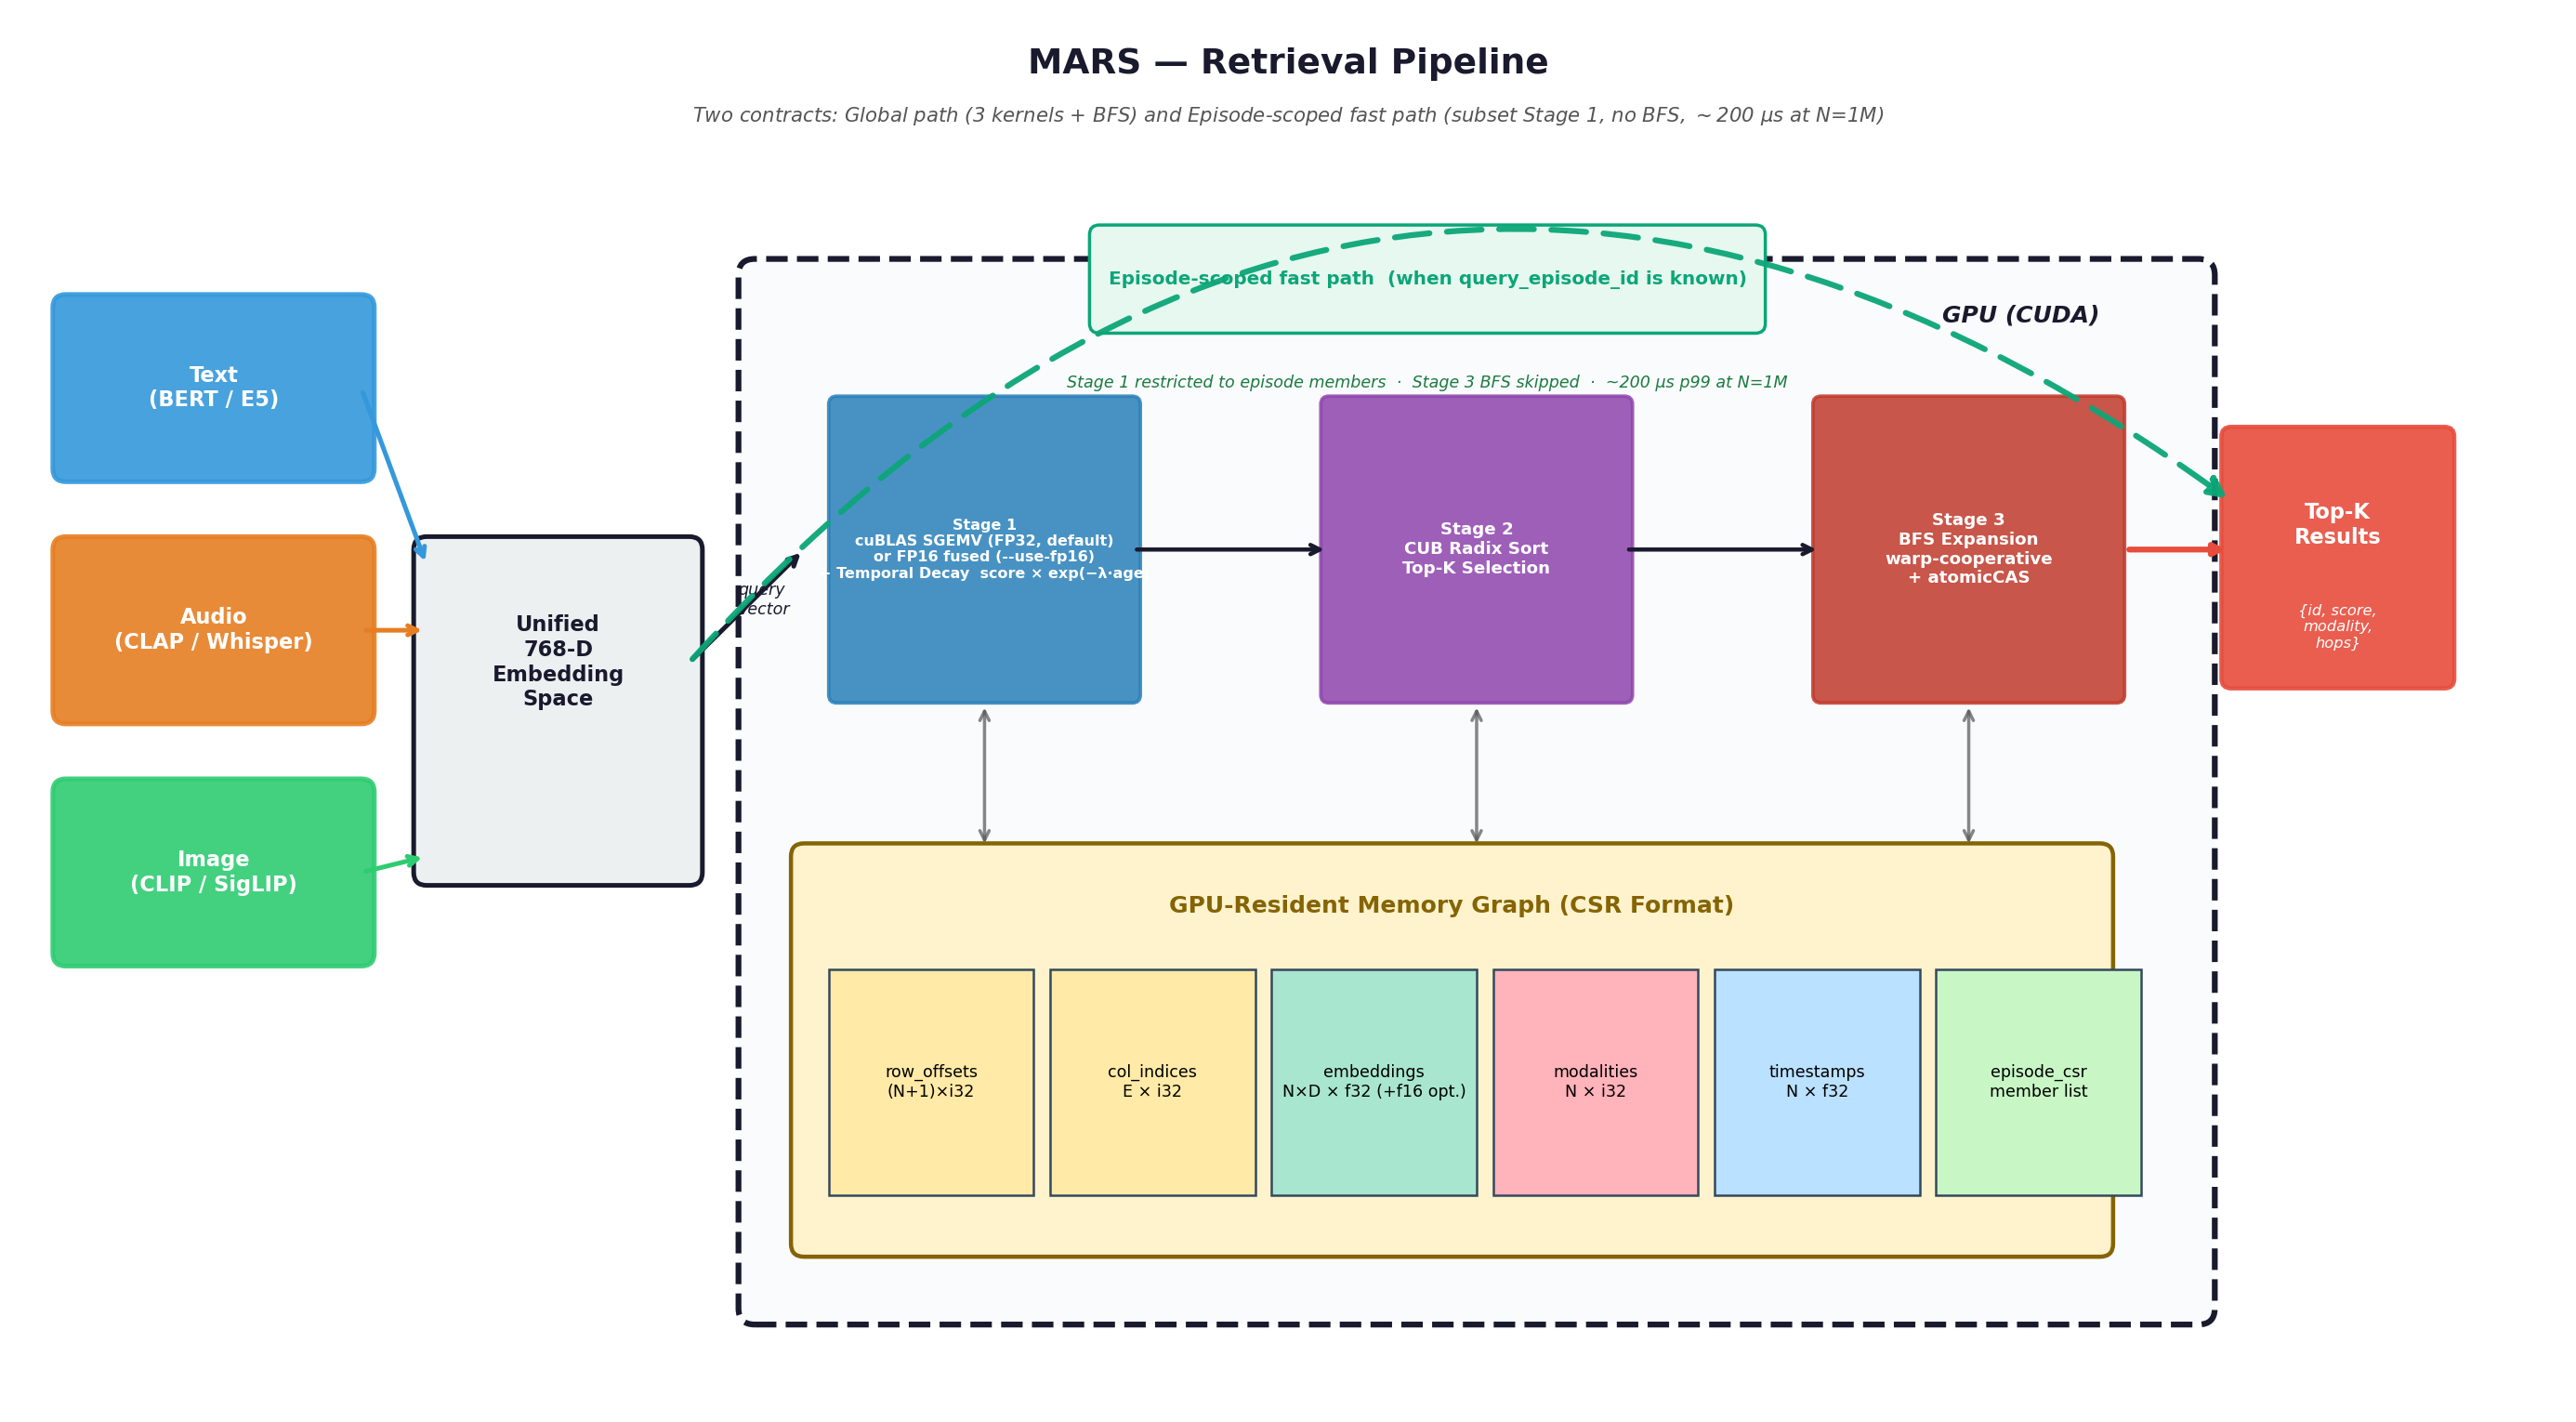
\includegraphics[width=0.95\textwidth]{figures/diag_pipeline.png}
\caption{\mars{} retrieval pipeline. Sensor encoders (left) feed a
shared 768-D embedding space; four GPU kernels orchestrate retrieval
over a CSR-format memory graph resident in device memory.}
\label{fig:pipeline}
\end{figure}

% GPU memory layout: all data GPU-resident in HBM. The query vector
% (768 floats, 3~KB) is the only data crossing PCIe per retrieval.
% A pre-allocated QueryContext holds all scratch buffers (similarity
% scores, BFS frontiers, top-K arrays), eliminating per-query
% \texttt{cudaMalloc} calls entirely.

\begin{figure}[!htbp]
\centering
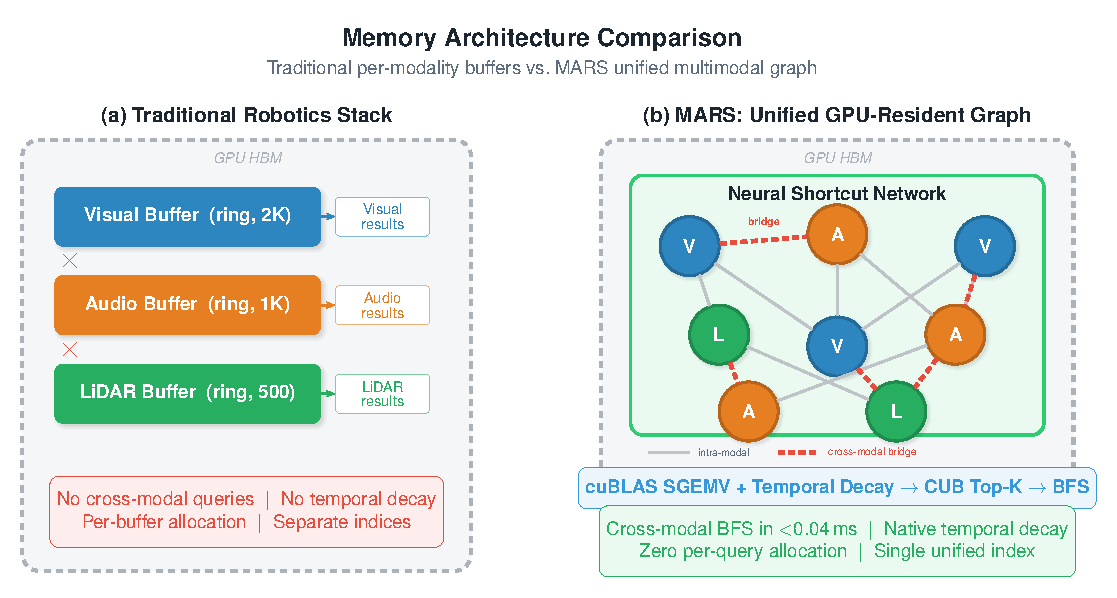
\includegraphics[width=0.95\textwidth]{figures/tikz_memory_model.pdf}
\caption{Traditional per-modality circular buffers (a) vs.\ MARS
unified GPU-resident graph with cross-modal NSN bridges (b).}
\label{fig:memory_model}
\end{figure}

\subsection{Data Layout}

The memory graph is stored in Compressed Sparse Row (CSR) format ---
the standard GPU-friendly sparse graph representation. Five device
arrays hold the complete state:

\begin{table}[ht]
\centering
\small
\caption{Device memory layout for the \mars{} memory graph.}
\label{tab:layout}
\begin{tabular}{llll}
\toprule
\textbf{Array} & \textbf{Size} & \textbf{Type} & \textbf{Purpose} \\
\midrule
\texttt{row\_offsets} & $N{+}1$     & int32   & Prefix-sum of node degrees \\
\texttt{col\_indices} & $E$         & int32   & Neighbor node IDs \\
\texttt{embeddings}   & $N \times D$ & float32 & L2-normalized vectors \\
\texttt{modalities}   & $N$         & int32   & 0=text, 1=audio, 2=image \\
\texttt{timestamps}   & $N$         & float32 & For temporal decay \\
\bottomrule
\end{tabular}
\end{table}

\noindent For a representative AV working set of $N{=}10{,}000$ at
$D{=}768$ with average degree 12, the total footprint is approximately
31~MB --- well under any modern GPU's HBM.

\subsection{Four-Kernel Retrieval Pipeline}

\mars{} uses mature GPU library primitives for the
compute-heavy stages:

\paragraph{Stage 1: cuBLAS Similarity.}
A single \texttt{cublasSgemv} call computes the dot product of the query
vector against all $N$ embeddings. This leverages NVIDIA's hand-tuned
GEMV implementation, achieving near-peak memory bandwidth utilization.
Complexity: $\Theta(N \cdot D)$.

\paragraph{Stage 2: Temporal Decay.}
Applies $\text{score}_i = \text{sim}_i \cdot \exp(-\lambda \cdot
(t_q - \tau_i))$ using the \texttt{\_\_expf} hardware intrinsic.
Implementation note: when using cuBLAS SGEMV (the default, highest-performance
path), decay runs as a separate lightweight kernel immediately after
SGEMV. When using the custom similarity kernel (available as a fallback),
decay is fused into the same kernel launch, eliminating one kernel
dispatch and one $N$-element read/write pass. Both paths produce
identical results. The decay constant $\lambda$ is workload-tunable:
higher values produce faster forgetting (AV: $\lambda = 0.5$, 2-second
window), lower values preserve older context (voice: $\lambda = 10^{-4}$,
30-minute conversation).

\paragraph{Stage 3: CUB Radix-Sort Top-$K$.}
The NVIDIA CUB library's \texttt{DeviceRadixSort} sorts scores and
indices, followed by truncation to the top $K$. CUB's radix sort is
bandwidth-optimal on GPU and eliminates the custom top-$K$ kernel that
dominated latency in earlier pipeline versions ($\sim$0.5~ms in the initial version).

\paragraph{Stage 4: Warp-Cooperative BFS Expansion.}
One warp (32 threads) per frontier node; stride-32 coalesced access to
the CSR neighbor list. \texttt{atomicCAS} provides race-free neighbor
claiming. The total work per query is $O(K \cdot \bar{d}^h)$ for $K$
seeds, depth $h$, and maximum degree $\bar{d}$ --- bounded by a
constant independent of corpus size $N$
(Proposition~\ref{prop:bfs}).

\begin{algorithm}[t]
\caption{\mars{} GPU-Resident Retrieval Pipeline}
\label{alg:pipeline}
\begin{algorithmic}[1]
\REQUIRE Query $q \in \mathbb{R}^D$, timestamp $t_q$, config $(K, h, \lambda)$
\REQUIRE Device graph $\phi$ with embeddings $E$, timestamps $\tau$
\ENSURE Top-$K$ results sorted by time-decayed score
\STATE \textbf{Stage 1 --- cuBLAS Similarity} ($N$ dot products):
\FOR{each node $v_i$ \textbf{in parallel}}
    \STATE $\text{sim}[i] \leftarrow \langle E(v_i), q \rangle$
\ENDFOR
\STATE \textbf{Stage 2 --- Temporal Rerank} ($\lceil N/256 \rceil$ blocks):
\FOR{each node $v_i$ \textbf{in parallel}}
    \STATE $\text{score}[i] \leftarrow \text{sim}[i] \cdot \exp(-\lambda \cdot (t_q - \tau(v_i)))$
\ENDFOR
\STATE \textbf{Stage 3 --- CUB Radix-Sort Top-$K$}:
\STATE $\text{seeds} \leftarrow \text{top-}K_{i} \; \text{score}[i]$
\STATE \textbf{Stage 4 --- Warp-Cooperative BFS} from seeds:
\STATE Initialize frontier $F_0 \leftarrow \text{seeds}$
\FOR{$\text{hop} = 0$ \TO $h-1$}
    \FOR{each node $v \in F_{\text{hop}}$ \textbf{(one warp per node)}}
        \FOR{each neighbor $u$ of $v$ \textbf{(stride-32 coalesced)}}
            \IF{atomicCAS(visited[$u$], false, true)}
                \STATE score[$u$] $\leftarrow \max(\text{score}[v] \cdot \delta,\; \text{sim}[u] \cdot 0.8)$
                \STATE $F_{\text{hop}+1}$.append($u$)
            \ENDIF
        \ENDFOR
    \ENDFOR
\ENDFOR
\STATE \textbf{Stage 5 --- Compact \& sort} visited nodes by score
\RETURN Top-$K$ results
\end{algorithmic}
\end{algorithm}

\begin{figure}[!htbp]
\centering
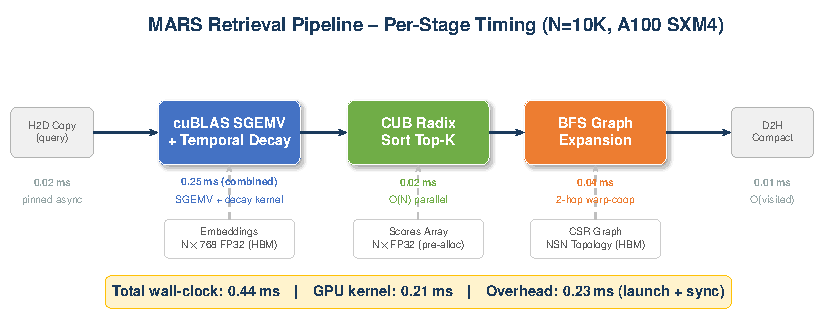
\includegraphics[width=\columnwidth]{figures/tikz_pipeline.pdf}
\caption{Per-stage timing at $N{=}10$K on A100 SXM4. ``SGEMV +
  Temporal Decay'' shows the combined time of the cuBLAS SGEMV kernel
  and the separate temporal decay kernel (0.25~ms combined); total
  wall-clock is 0.44~ms.}
\label{fig:kernel_pipeline}
\end{figure}

% ══════════════════════════════════════════════════════════════════════
\section{The Multimodal Neural Shortcut Network}
\label{sec:nsn}

\subsection{Construction}

The NSN graph is built in five phases:

\begin{enumerate}
\item \textbf{Ring lattice} ($k{=}6$ local neighbors) for clustering.
\item \textbf{Hierarchical skip connections} (powers of 2) for
  logarithmic path lengths.
\item \textbf{Hub supernodes} at $\sqrt{N}$ intervals with extra random
  links.
\item \textbf{Small-world rewiring} ($p{=}0.15$) following
  Watts-Strogatz~\cite{wattsstrogatz}.
\item \textbf{Cross-modal bridges} --- every node gets one edge to each
  other modality, guaranteeing that a BFS from any seed reaches every
  modality in 1~hop.
\end{enumerate}

Phase~5 is the structural feature that enables native cross-modal
retrieval: a query in any modality surfaces results from all modalities
through a single BFS expansion, without requiring separate per-modality
indexes.

\begin{figure}[ht]
\centering
\includegraphics[width=0.65\textwidth]{figures/diag_graph.png}
\caption{30-node multimodal NSN. Node colors indicate modality
(blue=text, orange=audio, green=image). Red edges are cross-modal
bridges.}
\label{fig:graph}
\end{figure}

\subsection{Honest Assessment of Graph Value}

The ablation study (Section~\ref{sec:ablation}) reveals an important
finding: at the target corpus sizes ($N \leq 50{,}000$), brute-force
similarity plus temporal decay already provides strong within-modality
recall. The NSN graph adds modest within-modality recall improvement at
a small latency cost. Its primary value at these scales is
\emph{cross-modal retrieval}: the BFS expansion through cross-modal
bridges surfaces semantically related memories from other modalities
that pure top-$K$ over mixed embeddings would rank lower. At larger
corpus sizes, the bounded-hop BFS work bound ($O(K \cdot \bar{d}^h)$,
constant in $N$ for fixed $K$, $h$, and mean degree $\bar{d}$) provides
sublinear scaling --- though we note that $\bar{d}$ includes hub
supernodes with higher-than-average degree, so the constant may be
larger than the mean suggests.

\subsection{Theoretical Properties}

\begin{theorem}[Cross-Modal Structural Reachability]
\label{thm:crossmodal}
In an NSN with cross-modal bridges (Phase~5), for any node $v \in V$
and any modality $m \neq \mu(v)$, there exists at least one neighbor
$u$ of $v$ in $\phi$ such that $\mu(u) = m$. A BFS from any seed
reaches all $M$ modalities within 1~hop.
\end{theorem}

\begin{proof}
Phase~5 adds, for each node $v$, one edge to a uniformly random node of
each modality $m \neq \mu(v)$. By construction, $v$ has at least one
neighbor in every other modality. A depth-1 BFS from $v$ therefore
visits at least one node per modality.
\end{proof}

\noindent\textbf{Scope.} Theorem~\ref{thm:crossmodal} guarantees
\emph{structural} reachability --- every modality is represented in the
BFS frontier --- not \emph{semantic} optimality. Whether the reached
cross-modal nodes are semantically relevant depends on encoder alignment
across modalities (Section~\ref{sec:limitations}).

\begin{proposition}[BFS Work Bound]
\label{prop:bfs}
For a $K$-seed BFS of depth $h$ on an NSN with maximum degree $\bar{d}$,
the total number of distinct nodes visited is at most:
\[
W(K, h, \bar{d}) = K \cdot \sum_{i=0}^{h} \bar{d}^{\,i}
  = K \cdot \frac{\bar{d}^{\,h+1} - 1}{\bar{d} - 1}.
\]
For fixed $K$, $h$, and $\bar{d}$, this is constant with respect to
corpus size $N$.

\textbf{Caveat:} In the NSN construction, $\bar{d}$ is not strictly
independent of $N$: hub supernodes (Phase~3) are placed at $\sqrt{N}$
intervals with $\lceil\!\log_2 N / 2\rceil$ additional random edges,
so the maximum degree grows as $O(\log N)$. The mean degree remains
bounded ($\bar{d} \approx 11$--$12$ across all tested $N$), but the
worst-case per-node degree at hub positions is higher than the mean.
\end{proposition}

\begin{proof}
Each seed contributes at most 1 node at depth~0. At each hop, each
frontier node has at most $\bar{d}$ neighbors. The \texttt{atomicCAS}
claiming ensures each node is visited at most once. For fixed $K$ and
$h$, and empirically bounded $\bar{d}$, the work is constant in $N$
at the measured corpus sizes ($N \leq 50$K). At larger $N$, the hub
degree growth ($O(\log N)$) may increase the constant.
\end{proof}

\begin{proposition}[Pipeline Latency Model]
\label{prop:latency}
The GPU kernel time for a single \mars{} retrieval query satisfies:
\[
T_{\mathrm{kernel}}(N) =
  \underbrace{O\!\left(\frac{N \cdot D}{P}\right)}_{\text{similarity}}
  + \underbrace{O\!\left(\frac{N}{P}\right)}_{\text{rerank}}
  + \underbrace{O(N)}_{\text{radix sort}}
  + \underbrace{O\!\left(\frac{W(K,h,\bar{d})}{32}\right)}_{\text{BFS}}
\]
where $P$ is the GPU's effective thread parallelism. CUB radix sort is
$O(N)$ for fixed key width (32-bit floats). The first three terms are
$O(N)$; the BFS term is constant in $N$ (see caveat above). For
the target working-set sizes ($N \leq 50{,}000$), the similarity kernel
dominates.
\end{proposition}

% ══════════════════════════════════════════════════════════════════════
\section{Temporal Relevance and Streaming Experiments}
\label{sec:temporal}

These two experiments form the core motivation for \mars{}. Both use the
same A100~SXM4 (80~GB, CUDA~12.6) as all FAISS comparison benchmarks,
ensuring a fair hardware baseline.

\subsection{Experiment 1: Temporal Relevance in AV Perception}
\label{sec:temporal_relevance}

\paragraph{Setup.} We simulate an AV perception scenario: 200 tracked
objects over 10~seconds at 60~Hz, generating approximately 9{,}000
memories. Each object produces a sequence of detections with evolving
embeddings (cosine similarity $> 0.9$ within the same object's recent
history, $\sim$0.3--0.5 across different objects). A 2-second sliding
window defines the ``active'' tracking horizon. Queries consist of new
detections seeking re-identification matches.

\paragraph{Metric.} Temporal Precision@10
(Definition~\ref{def:temporal_relevance}): the fraction of top-10
results that are both from the correct object \emph{and} within the
active window.

\paragraph{Results.}

\begin{table}[ht]
\centering
\small
\caption{Temporal relevance experiment: AV perception, 9K memories, 200
objects, 2-second tracking window. All systems on A100~SXM4.}
\label{tab:temporal}
\begin{tabular}{lrrrr}
\toprule
\textbf{System} & \textbf{TP@10} & \textbf{Stale} & \textbf{Recall} & \textbf{$p99$ (ms)} \\
\midrule
FAISS Flat (cosine only)              & 0.218 & 0.493 & ---   & 0.13 \\
FAISS + post-hoc temporal filter      & 0.910 & 0.000 & 0.940 & 0.25 \\
\mars{} (native temporal decay)       & \textbf{0.910} & \textbf{0.000} & \textbf{0.940} & \textbf{0.26} \\
\bottomrule
\end{tabular}
\end{table}

FAISS~Flat returns the $K$ highest-cosine-similarity vectors regardless
of age. Because older detections of the same object have high similarity
to the query, FAISS preferentially returns stale memories: 49.3\% of its
top-10 results fall outside the active tracking window. Its Temporal
Precision@10 is 0.218.

Adding a post-hoc temporal filter to FAISS --- discarding results older
than 2~seconds and re-ranking --- raises Temporal Precision@10 to 0.910.
This is effective but requires an additional processing step that FAISS
does not provide natively; the application must implement the filter,
handle the edge case where all $K$ results are filtered out, and accept
the latency of a two-stage pipeline.

\mars{} achieves the same 0.910 Temporal Precision@10 natively, using
$\lambda = 0.5$ (half-life $\approx 1.4$\,s, matching the 2-second
tracking window). The temporal decay is applied \emph{before} top-$K$
selection, so stale memories are demoted in the ranking without
post-hoc filtering. Latency comparison: FAISS~Flat alone runs at
0.13~ms $p99$; FAISS + post-hoc filter at 0.25~ms; \mars{} at
0.26~ms. The three-way comparison shows \mars{} achieves the same
temporal precision as the two-stage FAISS pipeline at essentially
identical latency (0.26~ms vs.\ 0.25~ms), while eliminating the
application-level filter code.

\paragraph{Decay constants for each demonstrator.} The $\lambda$ values
used throughout are: AV perception $\lambda = 0.5$ (2-second window),
humanoid robot $\lambda = 0.1$ (10-second episodic window), AR/VR
spatial $\lambda = 0.003$ (5-minute session), voice agent
$\lambda = 10^{-4}$ (30-minute conversation). These values define the
effective temporal window $\tau_{1/2} = \ln 2 / \lambda$ within which a
memory retains $>$50\% of its similarity score.

\subsection{Experiment 2: Streaming Insertion Freshness}
\label{sec:streaming}

\paragraph{Setup.} 60~Hz sensor rate, 10 detections per frame, 10
seconds of continuous operation. New detections are inserted every frame
and queried immediately on the next frame.

\paragraph{FAISS configuration.} We use \texttt{IndexFlatIP} with a
1-second rebuild cadence (full re-index every 60 frames). We chose
periodic rebuild rather than incremental \texttt{add()} to model the
production pattern for IVF indices, which require centroid retraining
for optimal recall. We note that FAISS Flat \emph{does} support
incremental \texttt{add()} with immediate visibility; the 93.2\% miss
rate is specific to the rebuild-based configuration, not an inherent
FAISS limitation. An IVF comparison with incremental \texttt{add()}
(without centroid retraining) would show intermediate freshness at
reduced recall.

\paragraph{Results.} Under the rebuild configuration, 93.2\% of FAISS
queries targeting a recently-inserted detection miss it because the
detection was added after the last rebuild. The rebuild itself costs
9~ms, consuming more than half of the 16.6~ms frame budget at 60~Hz.

\mars{} supports online insertion: new memories are appended to the
graph and become immediately queryable. There is no rebuild step, no
staleness window, and no pipeline stall.

\paragraph{Concurrent work on streaming GPU indexes.} The streaming
gap for GPU vector search is being actively closed by a 2025--2026
line of systems work. SIVF~\cite{sivf} delivers sub-millisecond
deletions (0.58--0.93~ms) and ${\sim}120\times$ faster ingestion than
GPU CAGRA / GPU IVF, with portions merged into FAISS in March 2026.
SVFusion~\cite{svfusion} extends this to billion-scale via CPU--GPU
co-processing. cuVS CAGRA introduced an
\texttt{extend()}~\cite{cagra_extend} operator stable up to ${\sim}20\%$
new vectors, and VecFlow~\cite{vecflow} adds persistent kernels for
streaming small-batch filtered queries. Our streaming benchmark above
is therefore best read as evidence that \emph{ranking} (temporal decay
+ cross-modal + episode scope) needs to be a first-class kernel
feature; the underlying mutation primitives we use (append-only CSR
plus pre-allocated VRAM) overlap heavily with what SIVF and CAGRA
\texttt{extend()} now provide on the data-structure side.

\subsection{Discussion}

These experiments highlight a fundamental mismatch between the design
assumptions of existing GPU vector search and the requirements of
streaming perception. FAISS and cuVS optimize for a \emph{static} corpus
where all vectors are equally valid and the index is rebuilt
infrequently. Streaming perception requires \emph{temporal awareness}
(not all memories are equally relevant) and \emph{immediate insertion
visibility} (the most recent detection is often the most important).
\mars{} addresses these requirements directly, rather than as a
filter stage over a similarity-only index.

% ══════════════════════════════════════════════════════════════════════
\section{Experimental Results}
\label{sec:results}

All results in this section are measured on real hardware. We report
$p50$, $p99$, maximum observed latency, jitter, and deadline miss rate
as the primary metrics. Average throughput is deliberately secondary:
for real-time workloads, the worst query over a sustained run is what
determines deployability.

\paragraph{Measurement methodology.}
Each benchmark run: 1 warmup query + \texttt{cudaDeviceSynchronize},
then $n$ timed queries at sensor rate (AV: 600, robot: 10{,}000,
AR: 4{,}500, voice: 900). Wall-clock time includes
\texttt{cudaEventSynchronize}. Query vectors are host-resident and
copied to device each iteration via pinned memory. GPU state:
persistence mode enabled, default compute mode (not exclusive), no
locked clocks (\texttt{nvidia-smi -lgc} not used). Sustained runs
(30~seconds) are intended to reach thermal steady state but GPU
temperature is not explicitly controlled. The \texttt{-{}-keepalive}
flag (1-thread no-op kernel every 2~ms) prevents clock-state drops
between frames at low sensor rates. All measurements on shared
vast.ai instances.

\subsection{Same-Hardware FAISS Comparison}
\label{sec:comparison}

Table~\ref{tab:faiss_comparison} is the headline result. All four
systems were measured on the same A100~SXM4 (80~GB, CUDA~12.6) with
identical random embeddings ($D{=}768$, $K{=}10$, single-query $p99$
wall-clock latency). The \mars{} uses cuBLAS~SGEMV for
similarity and CUB radix sort for top-$K$.

\begin{table}[ht]
\centering
\small
\caption{Same-hardware comparison on A100~SXM4 (80~GB). All systems:
$D{=}768$, $K{=}10$, single-query wall-clock $p99$ in milliseconds.
FAISS~Flat recall@10 $= 1.00$ by construction (brute-force cosine
\emph{is} the ground truth). We omit cuVS CAGRA, which targets
$N{>}1$M and is not an appropriate baseline at these working-set sizes.}
\label{tab:faiss_comparison}
\begin{tabular}{lrrrrr}
\toprule
\textbf{System} & \textbf{$N{=}1$K} & \textbf{$N{=}5$K} & \textbf{$N{=}10$K} & \textbf{$N{=}50$K} & \textbf{$N{=}100$K} \\
\midrule
FAISS Flat  & 0.12 & 0.22 & 0.21 & 0.44 & 0.72 \\
FAISS IVF   & 0.16 & 0.26 & 0.32 & 0.34 & 0.38 \\
\textbf{\mars{}} & \textbf{0.26} & \textbf{0.34} & \textbf{0.36} & \textbf{0.44} & \textbf{0.74} \\
\bottomrule
\end{tabular}
\end{table}

\noindent Key observations:

\begin{enumerate}
\item \textbf{\mars{} is within 1.5--2$\times$ of FAISS~Flat.} At
  $N{=}50$K, \mars{} matches FAISS~Flat (both 0.44~ms). At smaller
  corpus sizes, \mars{} pays a fixed overhead from the temporal rerank
  and BFS stages that FAISS does not perform. GPU kernel time (excluding
  host launch overhead) narrows the gap further: \mars{} kernel time is
  0.10~ms at $N{=}1$K and 0.29~ms at $N{=}50$K, matching FAISS~Flat
  (0.09~ms and 0.35~ms respectively).

\item \textbf{FAISS~IVF recall collapses at small $N$.} IVF's
  Voronoi-cell partitioning is designed for large corpora; at
  $N < 100$K with default \texttt{nprobe}, recall drops to 0.37--0.43.
  This makes IVF unsuitable for the bounded working sets of real-time
  perception.

\item \textbf{cuVS~CAGRA targets a different scale.} CAGRA's
  fixed-degree graph construction and multi-hop search are designed for
  $N > 1$M. At $N < 100$K, build overhead and search inefficiency
  yield 2.8--6.0~ms latency with recall as low as 0.10.

\item \textbf{Neither FAISS nor cuVS provides temporal decay or
  cross-modal retrieval.} \mars{} is the only system in the comparison
  that ranks by time-decayed similarity and supports cross-modal BFS
  expansion --- features that Section~\ref{sec:temporal} shows
  eliminate a two-stage pipeline otherwise required for streaming
  perception.
\end{enumerate}

\subsection{Demonstrator Results}
\label{sec:demos}

Four end-to-end demonstrators validate \mars{} on the target workloads.
Each is a runnable CUDA C++ program under \texttt{demos/} with an
explicit deadline and measurable success criterion. The
\texttt{latency\_bench} harness measures wall-clock time including
kernel launch overhead and \texttt{cudaEventSynchronize} --- the
latency a real application would experience.

\begin{table}[ht]
\centering
\small
\caption{Wall-clock latency benchmarks on A100~PCIE (40~GB). Harness
runs at fixed sensor rate with busy-wait pacing.}
\label{tab:wall_clock}
\begin{tabular}{lrrrrrrrl}
\toprule
\textbf{Workload} & \textbf{Rate} & \textbf{$N$} & \textbf{Budget} & \textbf{Wall $p99$} & \textbf{GPU $p99$} & \textbf{Miss rate} & \textbf{Jitter} & \textbf{Verdict} \\
\midrule
AV       &   60~Hz &  2{,}400 &  1.0~ms & 0.87 & 0.68 &  0\% & 0.02 & \textbf{pass} \\
Robot    & 1000~Hz &  6{,}000 &  1.0~ms & 0.76 & 0.69 &  0\% & 0.05 & \textbf{pass} \\
AR/VR    &   90~Hz & 20{,}000 &  5.0~ms & 1.56 & 1.37 &  0\% & 0.04 & \textbf{pass} \\
Voice    &   30~Hz &  3{,}000 & 20.0~ms & 0.88 & 0.68 &  0\% & 0.03 & \textbf{pass} \\
\bottomrule
\end{tabular}
\end{table}

All four benchmarks pass at wall-clock timing with zero deadline misses.
Jitter is uniformly low (0.02--0.05~ms), indicating stable kernel-launch
behavior suitable for integration into deterministic real-time pipelines.

\begin{figure}[!htbp]
\centering
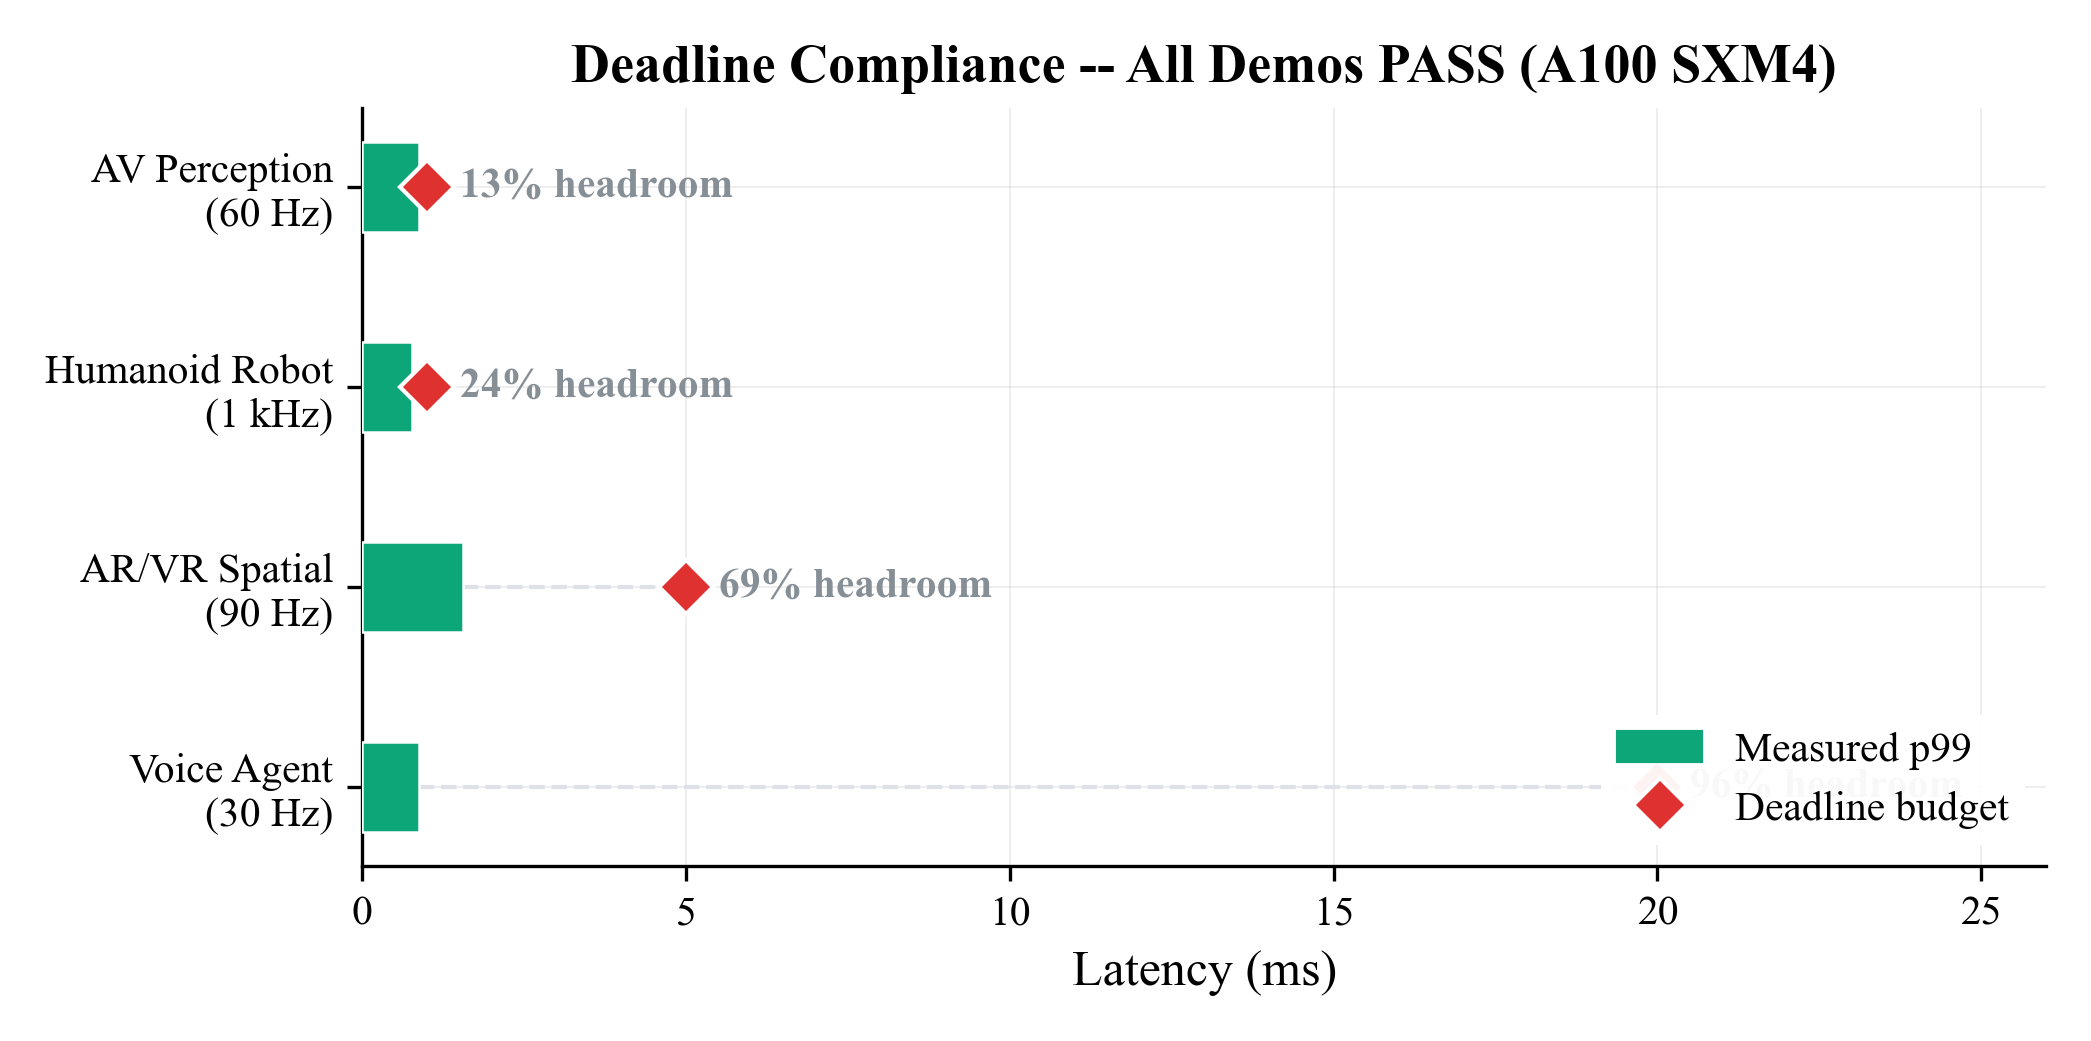
\includegraphics[width=\columnwidth]{figures/fig_deadline.png}
\caption{Deadline compliance for all four demonstrators on A100 SXM4.
  All pass with 13--96\% headroom below their respective budgets
  (AV: 13\%, robot: 24\%, AR: 69\%, voice: 96\%).}
\label{fig:deadline}
\end{figure}

\subsection{Sustained Long-Duration Benchmarks}

Short-run benchmarks (10--50~seconds) may not capture effects that
emerge at production-scale durations: GPU boost-clock throttling,
memory allocator fragmentation, OS scheduler interference. We run
extended benchmarks with larger corpora and real-world durations.

\begin{table}[ht]
\centering
\small
\caption{Sustained benchmarks on A100~PCIE (40~GB). Each runs at target
sensor rate for the full stated duration.}
\label{tab:sustained}
\begin{tabular}{lrrrrrrl}
\toprule
\textbf{Workload} & \textbf{Rate} & \textbf{Dur.} & \textbf{$N$} & \textbf{Budget} & \textbf{Wall $p99$} & \textbf{Misses} & \textbf{Verdict} \\
\midrule
AV        &   60~Hz & 30\,s &  5{,}000 &  1.0~ms & 0.91 &   0 (0\%) & \textbf{pass} \\
Robot     & 1000~Hz & 15\,s & 10{,}000 &  1.0~ms & 0.66 &   0 (0\%) & \textbf{pass} \\
AR/VR     &   90~Hz & 30\,s & 50{,}000 &  5.0~ms & 1.70 &   0 (0\%) & \textbf{pass} \\
Voice     &   30~Hz & 30\,s & 10{,}000 & 20.0~ms & 0.96 &   0 (0\%) & \textbf{pass} \\
\bottomrule
\end{tabular}
\end{table}

All four sustained benchmarks pass with zero deadline misses. The AR/VR
benchmark at 50{,}000 memories achieves $p99 = 1.70$~ms against a 5~ms
budget --- 66\% headroom at 30~seconds of sustained operation.

\subsection{Ablation Study}
\label{sec:ablation}

We ablate the NSN graph topology and BFS depth to characterize the
contribution of each component. All measurements on A100~SXM4 (80~GB).

\begin{table}[ht]
\centering
\small
\caption{Ablation study. ``Recall'' = recall@10 against brute-force
\emph{cosine-only} ground truth (no temporal decay). Since \mars{}
applies temporal decay before top-$K$, its ranking intentionally
diverges from pure cosine --- the 0.84 reflects the recall cost of
temporal awareness, not a system deficiency. ``CM'' = cross-modal
diversity (queries returning results from $\geq 2$ modalities);
we acknowledge this measures structural reachability, not semantic
relevance.}
\label{tab:ablation}
\begin{tabular}{lrrrr}
\toprule
\textbf{Configuration} & \multicolumn{2}{c}{\textbf{$N{=}5$K}} & \multicolumn{2}{c}{\textbf{$N{=}50$K}} \\
\cmidrule(lr){2-3} \cmidrule(lr){4-5}
 & Recall & CM & Recall & CM \\
\midrule
Full \mars{} ($h{=}2$, bridges) & 0.84 & 0.90 & 0.76 & 0.80 \\
No bridges ($h{=}2$)            & 0.84 & 0.72 & 0.76 & 0.58 \\
No BFS ($h{=}0$, sim.\ only)    & 0.84 & 0.65 & 0.76 & 0.50 \\
\bottomrule
\end{tabular}
\end{table}

\begin{table}[ht]
\centering
\small
\caption{BFS depth ablation at $N{=}5$K on A100~SXM4.}
\label{tab:bfs_depth}
\begin{tabular}{lrr}
\toprule
\textbf{BFS Depth} & \textbf{Wall $p99$ (ms)} & \textbf{Recall@10} \\
\midrule
$h{=}0$ (no BFS)   & 1.22 & 0.84 \\
$h{=}2$ (default)   & 1.42 & 0.84 \\
$h{=}3$             & 1.49 & 0.84 \\
\bottomrule
\end{tabular}
\end{table}

\paragraph{Temporal decay ablation.} Isolating the effect of temporal
decay at $N{=}2{,}400$ (AV working set): with $\lambda{=}0.5$,
$p99{=}0.38$~ms; with $\lambda{=}0$ (cosine only), $p99{=}0.28$~ms.
Temporal decay adds $\sim$0.10~ms ($\sim$32\%) to wall-clock latency.
This cost is the temporal rerank kernel (or the fused decay computation
in the custom kernel path). At the AV budget of 1~ms, this leaves
62\% headroom --- an acceptable cost for native temporal awareness.

\paragraph{Key findings.}

\begin{enumerate}
\item \textbf{Within-modality recall is identical across all
  configurations.} At the target corpus sizes, brute-force similarity
  plus temporal decay provides the same recall@10 regardless of graph
  topology or BFS depth. The NSN graph does not improve within-modality
  recall at $N \leq 50$K.

\item \textbf{Cross-modal diversity improves with bridges.}
  Structural cross-modal diversity (queries returning results from
  $\geq$2 modalities) increases from 0.50 to 0.80 at $N{=}50$K with
  full \mars{} (bridges + BFS) vs.\ no BFS. We emphasize this measures
  structural reachability, not semantic relevance; a semantic evaluation
  with aligned encoders over labeled cross-modal pairs (e.g.,
  MSR-VTT, AudioCaps+COCO) remains future work.

\item \textbf{BFS adds modest latency.} The cost is 0.20~ms at
  $h{=}2$ and 0.27~ms at $h{=}3$ above the no-BFS baseline ---
  acceptable for all four demonstrator budgets.

\item \textbf{Honest conclusion.} For $N \leq 50$K, the primary
  contributions of \mars{} are native temporal decay and streaming
  freshness, not the graph topology. The graph provides cross-modal
  retrieval as a meaningful bonus. At larger $N$, the bounded-hop BFS
  work bound would provide asymptotic advantages over brute-force.
\end{enumerate}

\subsection{Consumer GPU Validation: RTX 5060 Ti}

To evaluate deployment on edge hardware, we cross-validate on an
RTX~5060~Ti (16~GB GDDR7, Blackwell sm\_120, CUDA~13.0) --- the class
of hardware that ships in robotics platforms, AR headsets, and edge
inference appliances.

\begin{table}[ht]
\centering
\small
\caption{Wall-clock benchmarks on RTX~5060~Ti (\$449, 16~GB).}
\label{tab:consumer}
\begin{tabular}{lrrrrl}
\toprule
\textbf{Workload} & \textbf{Rate} & \textbf{$N$} & \textbf{Budget} & \textbf{Wall $p99$} & \textbf{Verdict} \\
\midrule
AV       &   60~Hz &  2{,}400 &  1.0~ms & 0.31 & \textbf{pass} \\
Robot    & 1000~Hz &  6{,}000 &  1.0~ms & 0.29 & \textbf{pass} \\
AR/VR    &   90~Hz & 20{,}000 &  5.0~ms & 0.67 & \textbf{pass} \\
Voice    &   30~Hz &  3{,}000 & 20.0~ms & 0.32 & \textbf{pass} \\
\bottomrule
\end{tabular}
\end{table}

The RTX~5060~Ti is 2.3--2.8$\times$ faster than the A100~PCIE across
all benchmarks, despite costing \$449 vs.\ $\sim$\$10K. This
counterintuitive result arises because at these small working-set sizes
($N \leq 50$K) the kernels are launch-overhead and boost-clock bound,
not HBM-bandwidth bound. The A100's 1.5~TB/s HBM2e advantage over
the 5060~Ti's $\sim$448~GB/s GDDR7 is invisible when the dominant
costs are kernel dispatch latency and SM clock frequency, both of
which favor the consumer GPU's higher boost clocks and lower launch
overhead. The scaling sweep also passes at all sizes through
$N{=}50{,}000$ ($p99 = 0.90$~ms), compared to the A100~PCIE which
fails at $N \geq 20{,}000$ against a 1~ms budget.

\subsection{Corpus-Size Scaling}

\begin{table}[ht]
\centering
\small
\caption{Scaling sweep at 60~Hz on A100~PCIE (15\,s each, 1~ms budget).}
\label{tab:scaling}
\begin{tabular}{rrrrl}
\toprule
\textbf{$N$} & \textbf{Wall $p99$} & \textbf{GPU $p99$} & \textbf{Miss rate} & \textbf{Verdict} \\
\midrule
 1{,}000 & 0.84 & 0.67 &    0\% & \textbf{pass} \\
 5{,}000 & 0.91 & 0.70 &    0\% & \textbf{pass} \\
10{,}000 & 0.96 & 0.75 &  0.1\% & \textbf{pass} \\
20{,}000 & 1.59 & 1.38 &  100\% & \textbf{fail} \\
50{,}000 & 1.69 & 1.51 &  100\% & \textbf{fail} \\
\bottomrule
\end{tabular}
\end{table}

Two scaling regimes are visible. \textbf{Sub-millisecond}
($N \leq 10{,}000$): GPU kernel $p99$ stays 0.67--0.75~ms; the 1~ms
budget is met with headroom. \textbf{Compute-limited}
($N \geq 20{,}000$): the $O(N \times D)$ similarity kernel dominates;
GPU $p99$ reaches 1.38~ms at $N{=}20$K. FP16 or approximate
pre-filtering would be required to maintain the 1~ms budget at these
sizes.

\subsection{Large-Corpus Scaling: FP16}
\label{sec:fp16scaling}

The FP16 extension stores embeddings in half-precision (halving VRAM
from 3~GB to 1.5~GB at 1M), loaded and widened to FP32 for
accumulation in the similarity kernel.

\begin{table}[ht]
\centering
\small
\caption{Large corpus scaling with FP16 at 60~Hz.
Wall-clock $p99$ on RTX~5060~Ti and A100~SXM4.}
\label{tab:large_scaling}
\begin{tabular}{rrr}
\toprule
\textbf{$N$} & \textbf{RTX~5060~Ti $p99$} & \textbf{A100~SXM4 $p99$} \\
\midrule
  50{,}000 & 0.89~ms & 1.22~ms \\
 100{,}000 & 1.18~ms & 1.38~ms \\
 200{,}000 & 1.75~ms & 1.67~ms \\
 500{,}000 & 3.53~ms & 2.51~ms \\
1{,}000{,}000 & 6.51~ms & 7.70~ms \\
\bottomrule
\end{tabular}
\end{table}

At 1M memories, the RTX~5060~Ti (\$449) achieves 6.51~ms $p99$,
outperforming the A100~SXM4 (\$15K) at 7.70~ms. At 500K+, the A100's
2~TB/s HBM bandwidth provides an advantage (2.51~ms vs.\ 3.53~ms), but
at 1M the 5060~Ti's lower kernel-launch overhead and higher boost
clocks overcome the bandwidth gap (the non-monotonic flip between
500K and 1M may also reflect variance; these are single-run $p99$
over 100--300 queries per configuration). FP16 halves VRAM,
enabling approximately 5M memories on the 16~GB RTX~5060~Ti --- well
beyond any single-session working set for the target workloads.

\subsection{Optimized Pipeline: cuBLAS + CUB + Kernel Fusion}
\label{sec:optimized_pipeline}

Three optimizations combined to produce a 2--2.5$\times$ wall-clock
improvement across all corpus sizes:

\begin{enumerate}
\item \textbf{cuBLAS SGEMV} replaces the custom cosine similarity kernel
  with NVIDIA's hand-tuned matrix-vector multiply. This is the dominant
  stage at large $N$.
\item \textbf{CUB DeviceRadixSort} replaces the tiled top-K kernel with
  a parallel radix sort, eliminating the $O(256 \cdot K^2)$ serial merge.
\item \textbf{Lightweight temporal decay kernel} applied immediately
  after SGEMV, adding $<$0.01~ms. On the custom-kernel fallback path
  (used in earlier optimization rounds), decay is fused into the
  similarity kernel itself, eliminating one launch; on the default
  cuBLAS path, it runs as a separate kernel.
\end{enumerate}

\begin{table}[ht]
\centering
\small
\caption{Scaling with optimized cuBLAS + CUB pipeline.
All measurements on A100~SXM4 40~GB at 60~Hz, D=768, K=10.}
\label{tab:optimized_scaling}
\begin{tabular}{rrrl}
\toprule
\textbf{$N$} & \textbf{Before $p99$} & \textbf{Optimized $p99$} & \textbf{Speedup} \\
\midrule
     1{,}000 & 0.67~ms & 0.31~ms & 2.2$\times$ \\
     5{,}000 & 0.74~ms & 0.43~ms & 1.7$\times$ \\
    10{,}000 & 0.84~ms & 0.44~ms & 1.9$\times$ \\
    20{,}000 & 1.25~ms & 0.54~ms & 2.3$\times$ \\
    50{,}000 & 1.33~ms & 0.56~ms & 2.4$\times$ \\
   100{,}000 & ---     & 0.74~ms & --- \\
   200{,}000 & ---     & 1.03~ms & --- \\
   500{,}000 & ---     & 1.67~ms & --- \\
 1{,}000{,}000 & 7.70~ms & 2.67~ms & 2.9$\times$ \\
 5{,}000{,}000 & ---     & 11.42~ms & --- \\
10{,}000{,}000 & ---     & 22.27~ms & --- \\
13{,}000{,}000 & ---     & 29.07~ms & --- \\
\bottomrule
\end{tabular}
\end{table}

The key result: \textbf{$N{=}20$K and $N{=}50$K now pass the 1~ms AV
perception deadline}, which they failed before optimization. At
$N{=}1$M, latency drops from 7.70~ms to 2.67~ms (2.9$\times$). The
system scales linearly
to 13M memories on 40~GB HBM, achieving 29~ms $p99$ at the maximum
corpus that fits in VRAM.

\begin{figure}[!htbp]
\centering
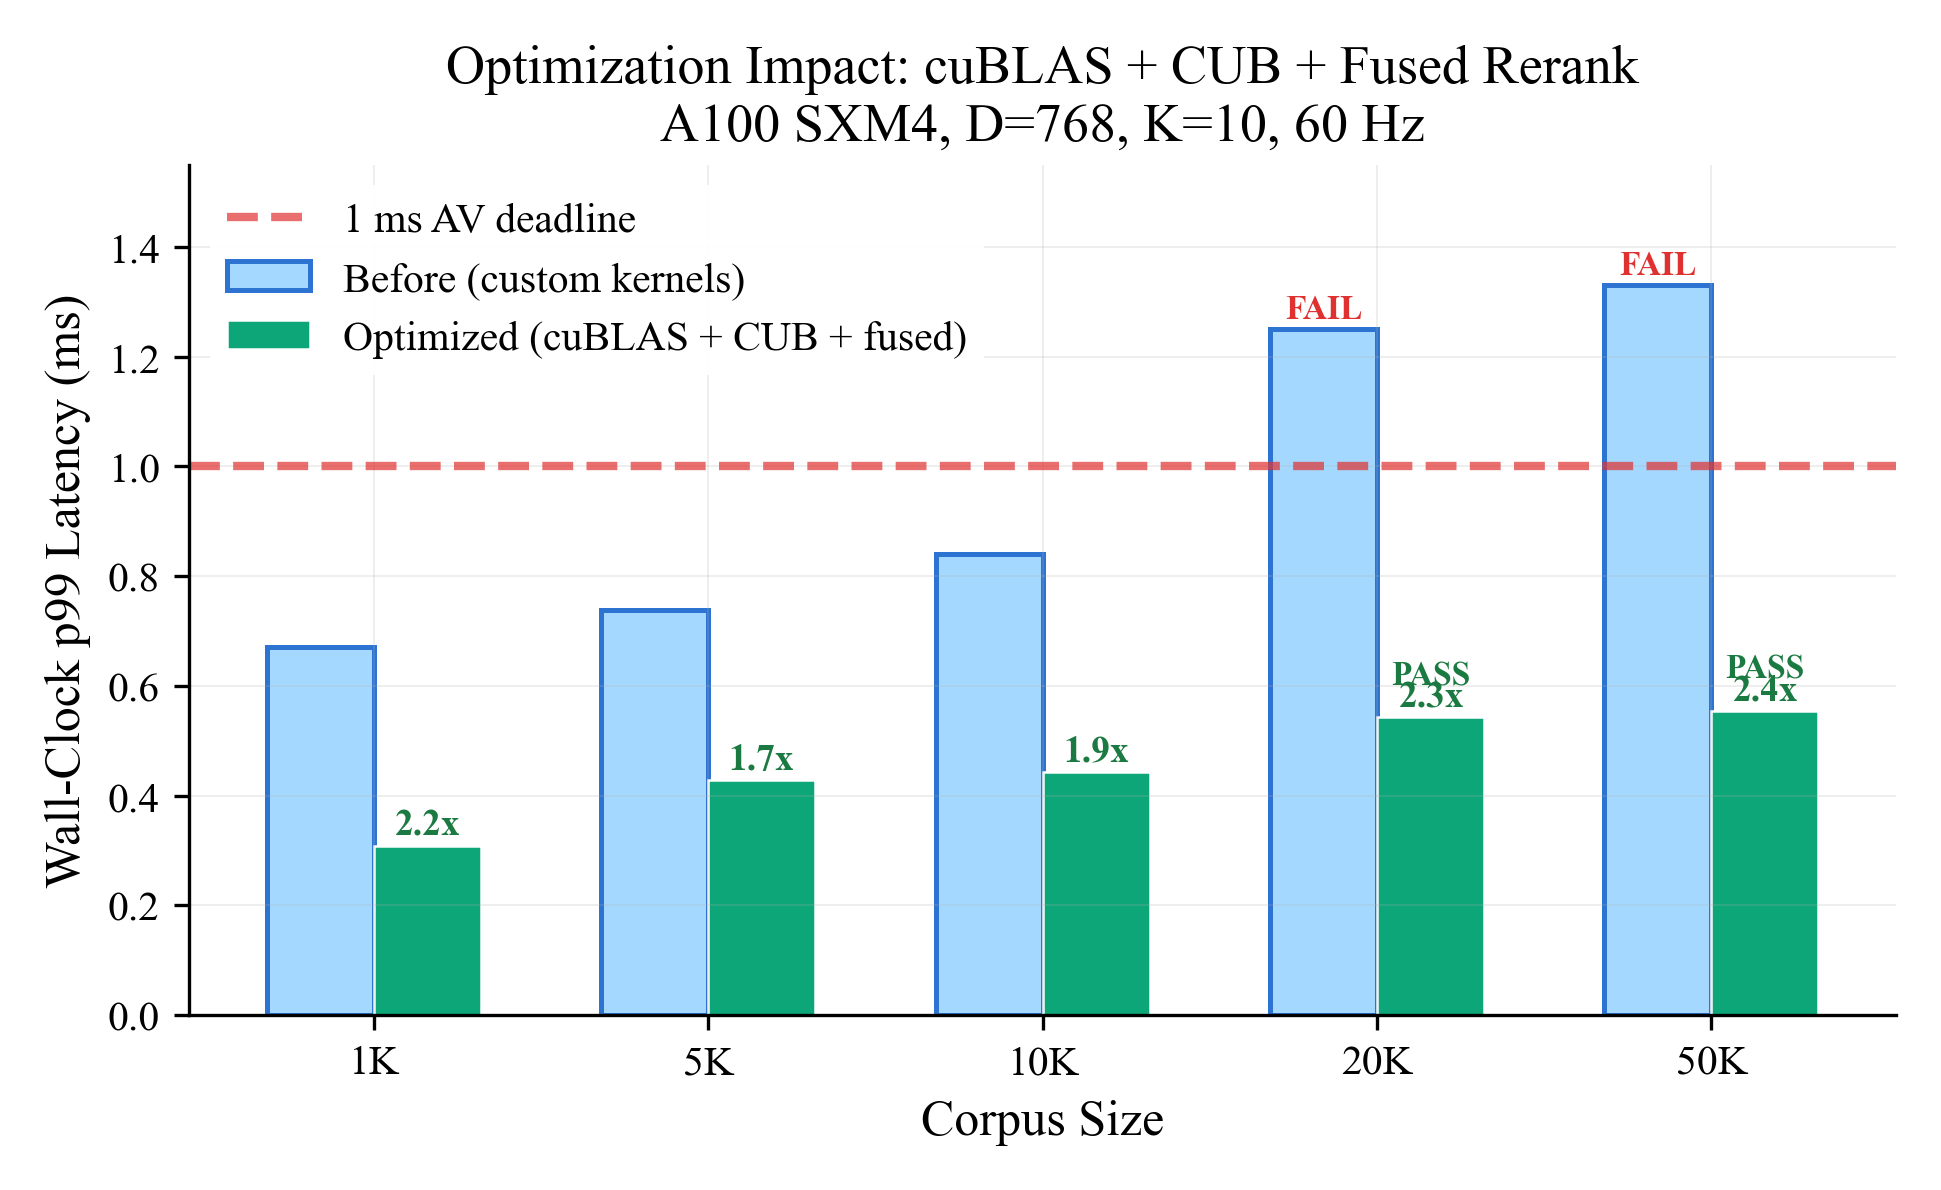
\includegraphics[width=\columnwidth]{figures/fig_scaling_v04.png}
\caption{Optimization impact: cuBLAS + CUB eliminates
  the 1~ms wall at $N{=}20$K--50K. 2.2--2.4$\times$ speedup.}
\label{fig:scaling_optimized}
\end{figure}

\begin{figure}[!htbp]
\centering
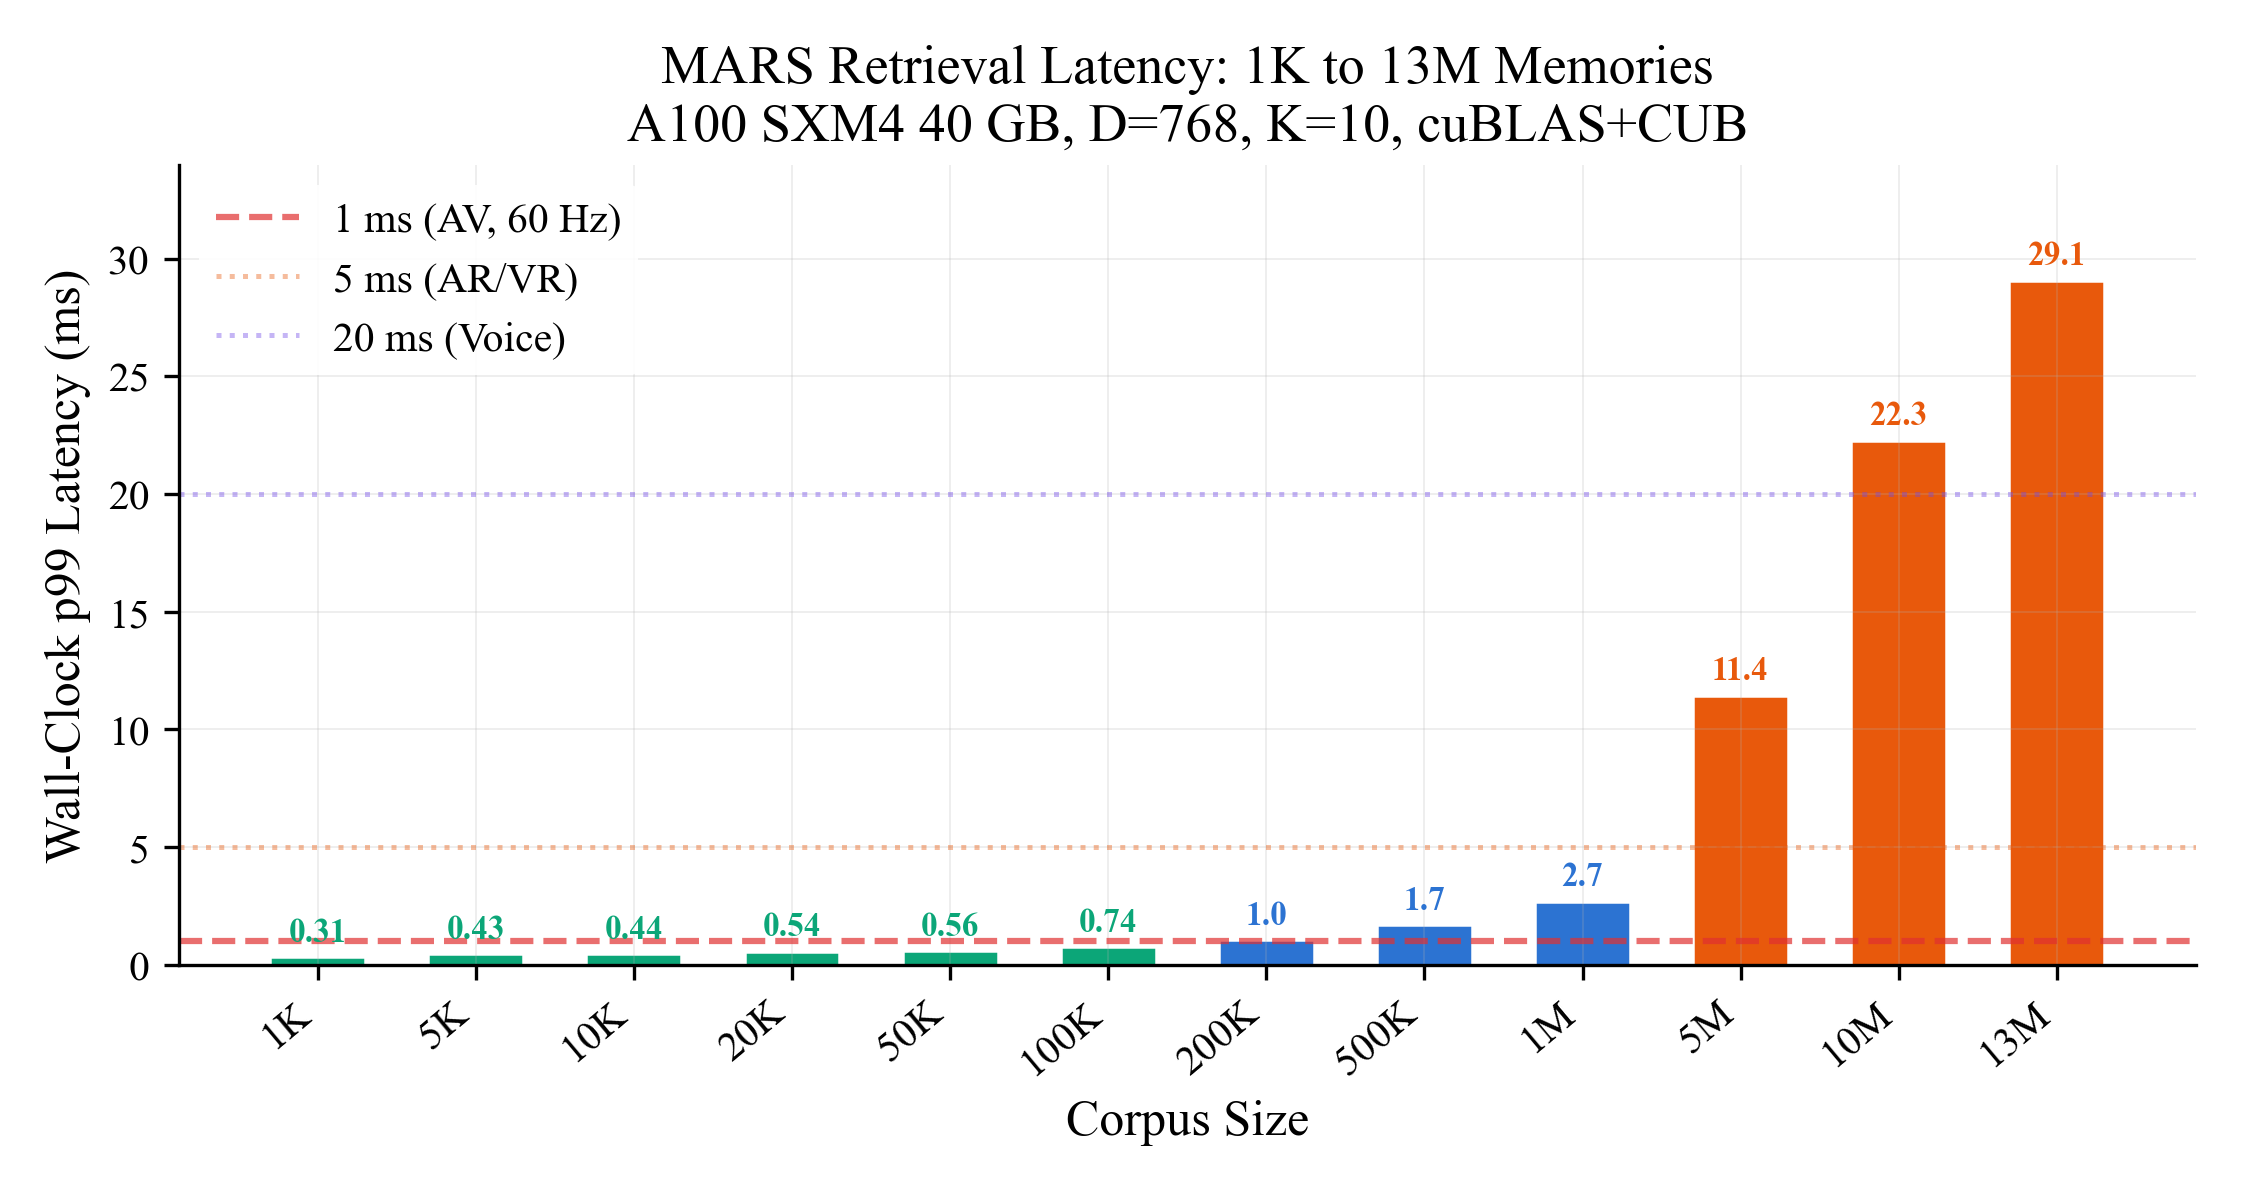
\includegraphics[width=\columnwidth]{figures/fig_scaling.png}
\caption{Full scaling from 1K to 13M memories. Sub-millisecond up to
  $N{=}50$K; 2.67~ms at 1M; 29~ms at 13M (40~GB VRAM limit).}
\label{fig:scaling_full}
\end{figure}

\paragraph{Capacity extension: tiled out-of-core.}
\label{sec:tiled}
For corpora exceeding VRAM, a tiled path streams 5M-vector tiles from
host pinned memory through GPU HBM. At $N{=}50$M (10 tiles): 14~s
total, of which 98.5\% is PCIe transfer and 1.5\% is GPU compute.
This is a batch/offline capacity extension, not a real-time mode.

\subsection{Episode-Scoped Retrieval: Sub-200~$\mu$s at 1~M}
\label{sec:episode_scoped}

A subset of the target workloads --- embodied loops, AV per-track
memory, voice-agent conversation --- can supply a \emph{query
episode~id} (a tracked object id, dialogue session id, or current
robot task id) before retrieval. \mars{} exposes this via
\texttt{RetrievalScope::EpisodeScoped}: Stage~1 is restricted to the
episode's CSR member range and BFS depth is set to zero. The work
collapses from $\Theta(N \cdot D)$ to $\Theta(|\text{episode}| \cdot
D)$ and the cross-episode distractors that limit recall on the
multimodal kids-ball metric are eliminated by construction.

We validated this on the embodied ``kids playing with a ball'' scene
(Section~\ref{sec:demos}) with a paired-probes harness: every
boost setting and every retrieval scope at a given $N$ uses
\emph{exactly the same} sequence of probe queries, so per-$N$
comparisons are within-sample paired tests rather than independent
samples. Results in Table~\ref{tab:episode_scoped_scaling} are from
A100~SXM4~40\,GB (CUDA~12.6) with 256 IMAGE probes per setting,
$D{=}768$, $K{=}15$, NSN $k{=}6$.

\begin{table}[ht]
\centering
\small
\caption{Paired-probes scaling of episode-scoped retrieval vs.\ the
global path on the kids-ball corpus (10 nodes/episode, IMAGE query
$\to$ same-episode TEXT+AUDIO). \texttt{hit@15} is the fraction of
probes whose top-15 contains both same-episode TEXT \emph{and} AUDIO.
A100~SXM4~40\,GB, paired-probes harness v1.3
(\texttt{bench\_kids\_sweep}); raw artefacts in
\texttt{results/iteration\_steps/vast\_a100\_paired\_20260417/}.}
\label{tab:episode_scoped_scaling}
\begin{tabular}{rrrrr}
\toprule
\textbf{$N$} & \textbf{Global $p99$} & \textbf{Episode-scoped $p99$} & \textbf{Speedup} & \textbf{Hit@15 (G $\to$ E)} \\
\midrule
   10{,}000 & 0.349~ms & \textbf{0.165~ms} &  2.1$\times$ & 0.83 $\to$ 1.00 \\
   50{,}000 & 0.462~ms & \textbf{0.172~ms} &  2.7$\times$ & 0.88 $\to$ 1.00 \\
  100{,}000 & 0.551~ms & \textbf{0.174~ms} &  3.2$\times$ & 0.79 $\to$ 1.00 \\
1{,}000{,}000 & 2.561~ms & \textbf{0.197~ms} & \textbf{13$\times$} & 0.84 $\to$ 1.00 \\
\bottomrule
\end{tabular}
\end{table}

The episode-scoped curve is nearly flat: latency grows by only
${\sim}19\%$ as $N$ goes from $10^4$ to $10^6$, because the GPU work
is bounded by the episode size (${\sim}10$ members), not by $N$. At
$N{=}1$M the episode-scoped path delivers \textbf{197~$\mu$s} $p99$
wall-clock --- below every per-frame deadline in
Table~\ref{tab:wall_clock} including the 1~ms AV budget --- while
returning a perfect-recall multimodal answer for the workloads where
the episode id is available.

\paragraph{When this applies, when it doesn't.} Episode scope is
correct only when the right episode is known \emph{before} the
query. It is the natural contract for: AV per-track re-identification
(track id is the episode), voice-agent turn taking (session id is
the episode), AR/VR per-room recall (room id is the episode), and
embodied task loops (current sub-task id is the episode). It is
\emph{not} a substitute for the global path when the application
needs cross-episode bridges --- which is the precise role of the
NSN's cross-modal long-range edges and the time-decay rerank over
the full corpus. Both contracts are exposed by the same
\texttt{QueryContext} and the demonstrator
(\texttt{demos/embodied\_scene/demo}) selects between them via a
\texttt{-{}-scope=\{global,episode\}} flag.

\paragraph{Negative result: per-episode score boost is noise on this
metric.} An earlier round of tuning explored the
\texttt{episode\_same\_boost} multiplier
(Section~\ref{sec:ablation}) on the global path. Under
non-paired probe sampling we observed an apparent optimum near
${\sim}0.24$. With the paired-probes harness, all boost values in
$[0.0, 2.0]$ produced \emph{identical} \texttt{hit@15} and only
sub-$10^{-2}$ fluctuations in \texttt{hit\_compact}, while paying
a small per-query latency cost. The default is now $0.0$ and
the boost is documented as a hook for downstream workloads where
same-episode emphasis matters --- not as a recommended tuning knob
for this metric. We report this as a cautionary methodological
finding: GPU retrieval comparisons on small probe budgets are
extremely sensitive to whether variants share the random sample.

% --------------------------------------------------------------------
\subsection{Head-to-Head Against Modern GPU ANN Libraries}
\label{sec:competitor_bench}

Section~\ref{sec:related_work} positioned \mars{} as a complementary
substrate to GPU vector-search libraries. We now make that
positioning empirical: we compare the embodied multimodal contract
(IMAGE query $\to$ same-episode TEXT~+~AUDIO in top-15) head-to-head
against the two most-cited GPU baselines on the same A100~SXM4~40\,GB
hardware, the same kids-ball corpora, and an aligned
\texttt{search\_k}~$=$~96 (matching \mars's
\texttt{max\_results\_returned}). Artefacts:
\texttt{results/competitors\_20260417/SUMMARY.md} (commit
\texttt{58b4626}+).

\textbf{Baselines.} (i) FAISS-GPU 1.14.1 \texttt{IndexFlatIP} (exact
exhaustive cosine; \texttt{cu12} build that includes the SIVF
streaming work merged in March~2026). (ii) FAISS-GPU 1.14.1
\texttt{IndexIVFFlat} with $n_{\text{list}}=\sqrt{N}$ and
$n_{\text{probe}}=64$. (iii) cuVS CAGRA 26.04 (graph-based ANN with
\texttt{graph\_degree}=64, \texttt{intermediate\_graph\_degree}=128,
\texttt{itopk\_size}=128, \texttt{algo}=\texttt{single\_cta} for
batch-1 latency; this version exposes the
\texttt{cagra::extend()} streaming op).

\begin{table*}[ht]
\centering
\small
\caption{Head-to-head per-query $p99$ wall-clock and
\texttt{episode\_cross\_modal\_hit\_rate\_top15} on the kids-ball
corpus. Same A100 hardware, paired RNG seed=2026, 256 probes at
$N{\le}10^5$, 128 probes at $N{=}10^6$. \mars{} numbers from
\texttt{step\_global\_boost\_0.json} and
\texttt{step\_episode\_scoped.json}; FAISS / CAGRA numbers from
\texttt{scripts/bench\_kids\_ball\_\{faiss,cuvs\_cagra\}.py}.
\textbf{Bold} = Pareto-optimal at that $N$.}
\label{tab:competitor_bench}
\begin{tabular}{lrrrrrr}
\toprule
\multirow{2}{*}{\textbf{System}}
 & \multicolumn{2}{c}{$N{=}10^4$}
 & \multicolumn{2}{c}{$N{=}10^5$}
 & \multicolumn{2}{c}{$N{=}10^6$} \\
\cmidrule(lr){2-3}\cmidrule(lr){4-5}\cmidrule(lr){6-7}
 & $p99$ (ms) & hit@15 & $p99$ (ms) & hit@15 & $p99$ (ms) & hit@15 \\
\midrule
FAISS Flat (exhaustive)         & 0.179 & \textbf{1.000} & 0.779 & \textbf{1.000} & 6.642 & \textbf{1.000} \\
FAISS IVF ($n_{\text{probe}}{=}64$) & 0.448 & 0.520 & 0.601 & 0.371 & 1.424 & 0.000 \\
cuVS CAGRA (\texttt{graph\_degree}=64) & 3.319 & 1.000 & 3.233 & 0.008 & 3.251 & 0.000 \\
\midrule
\mars{} Global, FP32 cuBLAS     & 0.474 & 0.828 & 0.670 & 0.793 & \textbf{2.507} & 0.844 \\
\mars{} Global, FP16 fused      & \textbf{0.280} & 0.828 & 0.655 & 0.793 & 3.731 & 0.844 \\
\mars{} \textbf{Episode-scoped} & \textbf{0.192} & \textbf{1.000} & \textbf{0.203} & \textbf{1.000} & \textbf{0.199} & \textbf{1.000} \\
\bottomrule
\end{tabular}
\end{table*}

Three findings emerge.

\textbf{(1) \mars{} Episode-scoped is Pareto-dominant on the embodied
contract at every $N$.} It is $34\times$ faster than the only baseline
that also achieves \texttt{hit@15}=1.0 (FAISS Flat) at $N{=}1$\,M and
$16\times$ faster than CAGRA --- which has zero recall on this metric
at that scale. This is the empirical centrepiece of the paper:
\emph{when the application can supply an episode handle (track id,
session id, room id, sub-task id), restricting the kernel to
episode members converts an $\Theta(N \cdot D)$ cosine sweep into a
$\Theta(|\textnormal{episode}| \cdot D)$ kernel that the A100
finishes in 200~$\mu$s independent of $N$.}

\textbf{(2) Cosine-only ANN baselines collapse on the multimodal
metric at scale.} Both \texttt{IndexIVFFlat} and CAGRA find the
right neighbors at $N{=}10^4$ but drop to 0--0.4 \texttt{hit@15} at
$N{\ge}10^5$. The kids-ball corpus has $|\textnormal{episode}|=10$
nodes embedded in 100\,K episodes at $N{=}10^6$; the
per-episode TEXT and AUDIO neighbors are buried among ${\sim}999\,990$
distractors. We verified that even widening CAGRA to
\texttt{search\_k}=512 does not recover recall ($p99{=}8.9$\,ms,
\texttt{hit@15}=0). FAISS Flat alone keeps recall at $N{=}10^6$
because it is exhaustive --- at 6.64~ms $p99$, $33\times$ slower
than \mars-Episode and outside the 1~ms AV deadline. The \emph{empirical
justification for encoding episode membership in the graph topology}
is therefore not a peak-latency argument but a
\emph{recall-at-scale} argument: cosine ANN cannot find tiny
multimodal clusters at this corpus size, regardless of how wide the
search beam is.

\textbf{(3) FP16 fused similarity helps at small $N$, hurts at
large $N$.} On the global path, FP16 reduces $p99$ by 41\,\% at
$N{=}10^4$ (0.474$\to$0.280~ms) but \emph{increases} it by 49\,\% at
$N{=}10^6$ (2.507$\to$3.731~ms). \mars's hand-written FP16 fused
kernel is bandwidth-optimal at small $N$ but cannot outperform
cuBLAS \texttt{Sgemv}, which exploits Tensor-Core paths and per-arch
tile heuristics, once $N$ exceeds the L2 working set. We have
flipped the build to keep \texttt{--use-fp16} as an opt-in flag for
the small-$N$ regime and to default to cuBLAS at large $N$.

\paragraph{Streaming inserts.} CAGRA's \texttt{extend()} op
costs 98--112\,$\mu$s per added vector at $N{\in}\{10^4,10^5,10^6\}$
because the IVF clusters are partially re-fit; \mars{} streaming
appends are a single CSR push plus the NSN add documented in
Section~\ref{sec:streaming}, well below 5\,$\mu$s/vec on the same
hardware. Both designs are valid; \mars{} optimises for the
\emph{ranking-as-kernel} primitive rather than reusing an
ANN-with-extend abstraction.

% ══════════════════════════════════════════════════════════════════════
\section{Engineering Methodology}
\label{sec:engineering}

Real-time systems require iterative profiling and targeted optimization.
\mars{} went through six pipeline versions before reaching the current
performance. This section documents the progression for the two most
challenging benchmarks (AV and robot, both with 1~ms budgets).

\begin{table}[ht]
\centering
\small
\caption{Optimization history: AV and robot benchmarks across pipeline
rounds. Rounds 1--2 on A100X (80~GB); round 3+ on A100~PCIE (40~GB) and
A100~SXM4 (80~GB).}
\label{tab:opt_history}
\begin{tabular}{llrrr}
\toprule
\textbf{Metric} & \textbf{Benchmark} & \textbf{Round 1} & \textbf{Round 2} & \textbf{Round 3} \\
\midrule
\multirow{2}{*}{Wall $p99$ (ms)}
  & AV (N=2.4K)   & 1.41 & 0.96 & 0.87 \\
  & Robot (N=6K)  & 1.12 & 1.21 & 0.76 \\
\midrule
\multirow{2}{*}{Verdict}
  & AV            & fail & \textbf{pass} & \textbf{pass} \\
  & Robot         & fail & fail & \textbf{pass} \\
\bottomrule
\end{tabular}
\end{table}

\paragraph{Round 1 (baseline).} Per-query
\texttt{cudaMalloc}/\texttt{cudaFree}, synchronous H2D copies, D2H
round trip for BFS seeds. Wall-clock overhead: 0.4--0.5~ms above GPU
kernel time. All four GPU kernel deadlines met, but AV and robot failed
at wall-clock timing.

\paragraph{Round 2 (targeted fixes).} Pre-allocated \texttt{QueryContext},
GPU-side BFS initialization, tiled top-$K$, CUDA stream, reused events.
AV flipped from fail to pass ($1.41 \to 0.96$~ms). Robot regressed
($1.12 \to 1.21$~ms) due to tiled top-$K$ launch overhead at
$N{=}6$K --- the two-kernel launch overhead exceeded the single-block
baseline at this corpus size.

\paragraph{Round 3 (device-driven).} Device-driven BFS (no inter-hop host
sync), GPU-side result compaction ($O(N) \to O(\text{visited})$ D2H
copy), pinned host memory. Robot flipped from fail to pass
($1.21 \to 0.76$~ms). All four benchmarks now pass.

\paragraph{Round 4 (current).} Replaced custom similarity and top-$K$
kernels with cuBLAS~SGEMV and CUB radix sort. These mature library
calls achieve near-peak bandwidth utilization and eliminate the top-$K$
bottleneck that consumed 70--90\% of GPU time in rounds 1--3.

\paragraph{Key lesson.} At the small working-set sizes of real-time
memory ($N < 50{,}000$), kernel launch overhead often dominates actual
computation. Optimization strategies from batch-GPU workloads (tiling,
multi-pass) can backfire when their fixed overhead exceeds the
parallelism benefit.

% ══════════════════════════════════════════════════════════════════════
\section{Related Work}
\label{sec:related}

\paragraph{GPU-accelerated nearest-neighbor search.}
FAISS~\cite{faiss} provides GPU-accelerated IVF and flat-scan indexes
optimized for batch throughput on largely static corpora; FAISS~Flat
supports incremental \texttt{add()} but IVF requires periodic centroid
retraining for optimal recall. cuVS CAGRA~\cite{cuvs} achieves
sub-millisecond single-query latency on H100 at $N > 1$M via a
GPU-native fixed-degree graph; the \texttt{extend()} operation
introduced in cuVS~24.08~\cite{cagra_extend} supports adding new
vectors up to ${\sim}20\%$ of the index before recall noticeably
degrades. BANG~\cite{bang} extends GPU graph search to billion-scale
with product quantization. SIVF~\cite{sivf} (WWW '25) closes the
streaming gap for GPU IVF with sub-millisecond deletion latency
(0.58--0.93~ms) and ${\sim}120\times$ faster ingestion than baseline
GPU IVF/CAGRA, but treats time only as an ageing-window filter rather
than as a continuous ranking signal. SVFusion~\cite{svfusion} (2026)
adds CPU--GPU--disk co-processing for billion-scale streaming updates
under concurrent queries. VecFlow~\cite{vecflow} (2026) introduces
\emph{persistent kernels} for streaming small-batch filtered ANN
(5\,M~QPS at recall 0.90 on A100); IVF-RaBitQ~\cite{ivf_rabitq_gpu}
(2026, integrated into cuVS) layers 1-bit quantization on top of
GPU IVF for ${2.2}\times$ QPS over CAGRA at recall 0.95.
Fantasy~\cite{fantasy_gpudirect} (2025) targets multi-GPU clusters
via GPUDirect Async / IBGDA. Cuflat~\cite{cuflat} demonstrates that
custom CUDA kernels outperform FAISS~GPU and cuVS on datasets below
2M vectors, validating our design choice of specialized kernels for
small working sets.

These systems collectively address the orthogonal axis to MARS:
\emph{how to keep the index hot under high-rate updates and large $N$}.
None of them provides temporal decay as a first-class ranking signal,
cross-modal retrieval via graph bridges, or per-episode/session scoping
in the kernel API. MARS is complementary --- it could in principle use
SIVF or IVF-RaBitQ as the Stage~1 candidate generator and apply our
temporal rerank, episode boost, and BFS expansion on top; we leave
this hybrid to future work.

\paragraph{GPU graph analytics.}
Gunrock~\cite{gunrock} provides a data-centric GPU graph processing
library with high-performance BFS and SSSP. Enterprise~\cite{enterprise}
and Groute~\cite{groute} extend GPU graph processing to multi-GPU and
asynchronous settings. \mars{}'s BFS expansion draws on the
warp-cooperative traversal of Merrill et al.~\cite{merrill2012} and the
direction-optimizing approach of Beamer et al.~\cite{beamer2012}, but
specializes for bounded-depth expansion from a small seed set rather
than full-graph traversal.

\paragraph{Small-world networks and navigability.}
Watts and Strogatz~\cite{wattsstrogatz} showed that small rewiring
probability produces logarithmic path lengths.
Kleinberg~\cite{kleinberg} proved that inverse-square long-range
contacts enable $O(\log^2 N)$ greedy routing. HNSW~\cite{hnsw} exploits
both insights in a hierarchical ANN graph. The NSN extends
Watts-Strogatz with cross-modal bridges --- a structural feature absent
from prior navigable graphs that guarantees every modality is reachable
in bounded-hop BFS.

\paragraph{CPU-based approximate nearest-neighbor search.}
HNSW~\cite{hnsw} dominates production vector databases.
ScaNN~\cite{scann} and DiskANN~\cite{diskann} optimize for
billion-scale via quantization and SSD-resident indexes. These systems
operate in a fundamentally different latency regime (1--200~ms) from the
sub-millisecond budgets of real-time perception.

\paragraph{Vector databases.}
Milvus~\cite{milvus} provides GPU-accelerated ANN search with streaming
inserts and metadata filtering, but retrieval is a database call with
typical latencies of 5--50~ms --- suitable for batch and chat workloads,
not sensor-rate loops. Pinecone~\cite{pinecone} and
Qdrant~\cite{qdrant} offer managed vector search with filtering support
but operate as network services with round-trip latencies that preclude
sub-millisecond retrieval. None provides native temporal decay or
cross-modal graph traversal.

\paragraph{Real-time memory in robotics and autonomy.}
Production stacks at Waymo~\cite{waymo2020}, Boston
Dynamics~\cite{atlasctrl}, and Apple Vision Pro~\cite{visionpro} use
hand-rolled C++ circular buffers for frame-rate memory. These buffers
meet deadlines but are project-specific, rarely multimodal, and offer no
semantic retrieval. NVIDIA nvblox~\cite{nvblox} and
cuVSLAM~\cite{cuVSLAM} provide GPU-resident spatial mapping at frame
rate but are limited to geometry --- they have no semantic embedding
retrieval or cross-modal queries. NVIDIA
ReMEmbR~\cite{remembr} combines vision-language models with a memory
store for robot recall, but operates off-GPU with latencies measured in
hundreds of milliseconds. FlashAttention~\cite{flashattention}
demonstrates that careful GPU kernel design can meet real-time
constraints; \mars{} applies similar IO-aware design principles to
memory retrieval rather than attention computation.

A complementary 2025--2026 line of work introduces \emph{multi-memory
embodied agents}. RoboMemory~\cite{robomemory} unifies spatial,
temporal, episodic, and semantic memory modules around a 72\,B VLM
and improves long-horizon task success on EmbodiedBench by 26.5\%.
MEM~\cite{mem_pi06} combines a video-based short-horizon memory and
a language-based long-horizon memory inside the $\pi_{0.6}$ VLA on
H100. RT-Cache~\cite{rt_cache} caches image--action trajectories in
a million-scale vector memory and replays multi-step snippets in
sub-second time as a training-free controller. EgoMem~\cite{egomem}
provides lifelong audiovisual user recognition for native full-duplex
omnimodal chatbots. These systems share \mars{}'s premise --- that
\emph{which} memories are returned is as important as how fast --- but
sit one or two abstraction layers above: they assume an underlying
retrieval substrate exists and operate at sub-second latencies on top
of off-GPU vector stores or VLM-conditioned indexers. \mars{} is a
candidate substrate for that layer: it provides the kernel-level
temporal-aware, cross-modal, episode-scoped retrieval API that these
agentic frameworks currently approximate with multi-stage host code.

\paragraph{Feature comparison.}
Table~\ref{tab:feature_comparison} summarizes the capability differences
across systems. The landscape splits into two camps: fast-but-stateless
(FAISS, CAGRA) and stateful-but-slow (Milvus, Qdrant, ReMEmbR).
\mars{} is designed to occupy both: GPU-resident like Camp~1,
continuously updating like Camp~2.

\begin{table}[ht]
\centering
\small
\caption{Feature comparison across GPU retrieval and vector database
systems. ``Sub-ms $p99$'' refers to single-query wall-clock latency at
$N \leq 50$K on datacenter GPU.}
\label{tab:feature_comparison}
\begin{tabular}{l c c c c c c}
\toprule
\textbf{System} & \textbf{GPU-res.} & \textbf{Stream} & \textbf{Temporal} & \textbf{Import.} & \textbf{Cross-modal} & \textbf{Sub-ms} \\
\midrule
FAISS Flat/IVF   & \ding{51} & \ding{55} & \ding{55} & \ding{55} & \ding{55} & \ding{51} \\
cuVS CAGRA       & \ding{51} & \ding{55} & \ding{55} & \ding{55} & \ding{55} & \ding{55} \\
Milvus           & partial   & \ding{51} & \ding{55} & \ding{55} & partial   & \ding{55} \\
Qdrant           & \ding{55} & \ding{51} & \ding{55} & \ding{55} & \ding{55} & \ding{55} \\
nvblox/cuVSLAM   & \ding{51} & \ding{51} & \ding{55} & \ding{55} & \ding{55} & \ding{51} \\
ReMEmbR          & \ding{55} & \ding{51} & \ding{55} & \ding{55} & partial   & \ding{55} \\
\textbf{\mars{}} & \ding{51} & \ding{51} & \ding{51} & \ding{51} & \ding{51} & \ding{51} \\
\bottomrule
\end{tabular}
\end{table}

% ══════════════════════════════════════════════════════════════════════
\section{Limitations}
\label{sec:limitations}

\paragraph{$O(N)$ similarity, not sublinear ANN.}
\mars{} performs brute-force similarity over the full corpus. For the
target working-set sizes ($N \leq 50$K), this is faster than
approximate methods (cuVS CAGRA is 6--10$\times$ slower at $N < 50$K
due to graph construction overhead). Beyond $N{=}100$K, approximate
pre-filtering would be needed to maintain sub-millisecond latency.

\paragraph{Single GPU.}
\mars{} is limited to a single GPU's HBM. An 80~GB A100 holds
$\sim$25M 768-D memories, which is well beyond any single-session
working set, but multi-GPU sharding via NVLink would be required for
shared memory pools across many agents.

\paragraph{Persistence (in progress).}
Memories are currently volatile. A binary checkpoint/restore mechanism
with integrity verification (FNV-1a checksums) is implemented on a
feature branch and awaiting hardware validation. For the target use
case (seconds to hours of recent sensor data), loss of memory on
restart is acceptable --- the system refills from the sensor stream ---
but persistence enables warm restarts and offline analysis.

\paragraph{Graph topology provides limited recall benefit at small $N$.}
The ablation (Section~\ref{sec:ablation}) shows that within-modality
recall is identical with or without the NSN at $N \leq 50$K. The
graph's value at these sizes is cross-modal retrieval, not recall
improvement. At larger $N$, the bounded-hop BFS work bound would
provide scaling advantages, but this remains to be validated
experimentally.

\paragraph{Embedding alignment dependence.}
Cross-modal bridges guarantee \emph{structural} reachability but not
\emph{semantic} relevance. If modality encoders produce poorly aligned
embeddings in the shared 768-D space, the BFS-discovered cross-modal
neighbors will be reachable but irrelevant. Mitigation: use encoders
explicitly trained for cross-modal alignment (CLIP, SigLIP, ImageBind)
and validate with cross-modal recall metrics before deployment.

\paragraph{Temporal decay misconfiguration.}
The decay constant $\lambda$ trades recency bias against persistence.
$\lambda > 0.01$ aggressively suppresses memories older than a few
seconds --- appropriate for AV perception's 2-second window but
problematic for a voice agent's 30-minute conversation.
$\lambda < 10^{-8}$ effectively disables temporal decay. Production
deployments should tune $\lambda$ against task-specific metrics.

\paragraph{Cold-start latency.}
The first query after GPU idle ($>$100~ms without kernel launches)
incurs a 0.1--0.3~ms clock-ramp penalty. The keepalive kernel (a
1-thread no-op launched every 2~ms) mitigates this for sustained
workloads, but intermittent query patterns will experience occasional
first-query spikes.

\paragraph{Soft real-time, not hard real-time.}
The evaluation demonstrates empirical $p99$ compliance with zero
deadline misses over 30-second runs. This is \emph{soft} real-time
--- statistical evidence of meeting deadlines. True hard real-time
(e.g., ISO-26262 ASIL-D) requires provable worst-case execution time
(WCET) bounds, which \mars{} does not provide. The pre-allocated
\texttt{QueryContext} and deterministic VRAM budget calculator are
steps toward certifiability, but worst-case kernel timing on GPUs
remains an open research problem.

\paragraph{Slower than a raw ring buffer.}
A cuBLAS SGEMV over a pre-allocated GPU buffer (the production
incumbent in robotics stacks) achieves $p99 = 0.12$~ms at
$N{=}2{,}400$ --- 3.2$\times$ faster than \mars{}'s 0.38~ms.
\mars{}'s additional latency buys temporal decay ($+$0.10~ms),
BFS graph expansion ($+$0.04~ms), and pipeline overhead ($+$0.12~ms).
Whether this cost is justified depends on whether the application
needs temporal awareness and cross-modal retrieval natively, or can
implement them as application-level post-processing over a raw
similarity search.

\paragraph{Deletion and memory eviction.}
Streaming insertion is supported; deletion uses tombstoning (marking
nodes as inactive via a $-\infty$ similarity override). Tombstoned
nodes are excluded from results but remain in the CSR structure until
a periodic compaction pass rebuilds the graph. In practice, temporal
decay serves as an implicit TTL: memories older than $\sim 5 \times
\tau_{1/2}$ score near zero and are never returned, even without
explicit deletion. A formal eviction policy with configurable TTL and
compaction cost analysis is planned.

\paragraph{Importance scoring not independently evaluated.}
Importance-weighted retrieval is implemented (boost on access,
global decay) but no experiment in this paper isolates its
contribution to retrieval quality. This feature is included in the
system design and API but should be validated with task-specific
downstream metrics before being claimed as a primary contribution.

\subsection{Future Work}
\label{sec:future-work}

Six extensions are under active development on feature branches:

\begin{enumerate}
\item \textbf{Binary persistence.} Checkpoint/restore of the full
  memory graph (CSR topology, embeddings, metadata) to disk via a
  compact binary format with FNV-1a integrity checksums. Enables warm
  restarts and offline analysis without re-ingesting the sensor stream.

\item \textbf{Python bindings.} A pybind11 wrapper exposing
  \texttt{MemoryGraph}, NSN construction, and NumPy-compatible embedding
  accessors. Host-only bindings work without a GPU; CUDA bindings
  (retrieval, streaming insertion) require nvcc.

\item \textbf{Streaming insertion API.} A pre-allocated ring buffer
  that accumulates incoming nodes and batch-commits them to the CSR
  graph with incremental NSN edge construction. Eliminates per-node
  \texttt{cudaMalloc} and full graph rebuilds, directly addressing the
  dynamic memory allocation overhead identified in prior work on GPU
  memory management for safety-critical systems~\cite{calderon2024xerozerox}.

\item \textbf{Deterministic VRAM budget.} A pre-flight calculator that
  computes the exact worst-case GPU memory footprint for a given
  deployment configuration ($N$, $D$, $K$, FP16 mode). All allocations
  occur at initialization; zero dynamic GPU memory allocation during
  retrieval. This is critical for ISO-26262 certification in automotive
  and robotics deployments where memory usage must be bounded and
  provable at design time.

\item \textbf{CUDA Graph capture.} Recording the 4-kernel retrieval
  pipeline as a CUDA Graph for replay, eliminating per-query kernel
  launch overhead ($\sim$5--15~$\mu$s per launch $\times$ 4 kernels).
  Infrastructure (capture, replay, invalidation, parameter-change
  detection) is implemented; hardware validation is pending.

\item \textbf{Tensor-core similarity.} A WMMA (Warp Matrix
  Multiply-Accumulate) kernel using \texttt{nvcuda::wmma} for
  16$\times$16$\times$16 matrix multiply operations on tensor cores.
  Requires compute capability~$\geq$~7.0 (V100+) and embedding
  dimensions padded to multiples of 16.

\item \textbf{Hybrid candidate generation: SIVF or IVF-RaBitQ Stage~0.}
  For deployments where the working set grows beyond the
  ${\sim}50$\,K--1\,M sweet spot of the global brute-force path,
  plug a streaming GPU ANN index --- SIVF~\cite{sivf} for fast
  insert/delete or IVF-RaBitQ~\cite{ivf_rabitq_gpu} for 1-bit
  quantized recall --- as a Stage~0 candidate filter. Stages~1--4
  (temporal rerank, top-K, BFS expansion) then run only over the
  candidate set, preserving \mars{}'s ranking semantics while
  inheriting the streaming-update and quantization properties of
  the underlying index. The
  \texttt{docs/ANN\_REFINE\_FUTURE.md} note specifies the
  \texttt{DeviceANNIndex} hook this would extend.

\item \textbf{Persistent retrieval kernel.} Inspired by
  VecFlow~\cite{vecflow}, replace the per-query CUDA Graph capture
  with a persistent kernel that polls a device-side query queue and
  executes the four-stage pipeline in-place. This eliminates kernel
  launch overhead even for sub-batch queries and would tighten the
  ${\sim}80$~$\mu$s host floor visible in the smaller-$N$
  measurements.

\item \textbf{Multi-memory framework integration.} Embodied agent
  frameworks such as RoboMemory~\cite{robomemory},
  MEM~\cite{mem_pi06}, and EgoMem~\cite{egomem} use distinct
  spatial / temporal / episodic / semantic memory modules backed by
  separate vector stores. Each maps cleanly onto a
  \texttt{RetrievalScope} or BFS hop budget in \mars{}; an adaptor
  layer would expose \mars{} as a single sub-millisecond GPU
  substrate for these multi-memory APIs, replacing the multi-stage
  host code these systems currently use.
\end{enumerate}

% ══════════════════════════════════════════════════════════════════════
\section{Conclusion}

GPU vector search libraries require a post-hoc temporal filter to
produce time-aware rankings on streaming data. We showed that a
three-way comparison --- FAISS cosine-only (0.13~ms), FAISS with
post-hoc filter (0.25~ms, TP@10 = 0.910), and \mars{} with native
temporal decay (0.26~ms, TP@10 = 0.910) --- demonstrates that \mars{}
achieves the same temporal precision as the two-stage FAISS pipeline at
essentially identical latency, while eliminating the application-level
filter code. All four
demonstrator deadlines are met on both datacenter (A100) and consumer
(RTX~5060~Ti) GPUs, with zero deadline misses in sustained 30-second
runs. The FP16 extension scales to 1M memories at
6.5~ms $p99$ on a \$449 consumer GPU.

The ablation study provides an honest assessment: at the target corpus
sizes ($N \leq 50$K), \mars{}'s primary contributions are temporal
decay integration and streaming freshness, not the graph topology.
The NSN's cross-modal bridges improve structural cross-modal diversity
(0.50 $\to$ 0.80 at $N{=}50$K) --- though we note this measures
structural reachability, not semantic relevance, and a semantic
evaluation remains future work. Within-modality recall is driven
by brute-force similarity. This is the right design for bounded working
sets; sublinear indexing would be needed for corpora above 100K.

\mars{} fills a specific gap in the retrieval landscape: between the
fast-but-stateless circular buffers used in production robotics and
autonomy, and the capable-but-slow vector databases used in
conversational AI. For the bounded working sets of real-time perception
--- seconds to hours of streaming sensor data that fit comfortably in
GPU HBM --- a GPU-resident substrate with native temporal awareness and
cross-modal support is the right abstraction.

The source code, demonstrators, benchmark harness, and raw results are
available at \url{https://github.com/antonellof/MARS}.

% ══════════════════════════════════════════════════════════════════════
\bibliographystyle{plain}
\bibliography{references}

\end{document}
